\documentclass[a4paper,11pt]{article}
\usepackage{trymtex}
\addbibresource{frontmatter/ref.bib}


\begin{document}

\begin{titlepage}
    \newcommand{\HRule}{\rule{\linewidth}{0.5mm}}
    \center

    % Top section with logo
    \vspace*{1.5cm}  % Reduced from 2cm
    \begin{center}
        
\includegraphics[width=5cm]{frontmatter/TS_GooseLogo.png}
    \end{center}

    \vspace{1.5cm} 

    % Course code & title with modern styling

    {\color{ntnu-blue}\sffamily\Large TMA4180 \par}
    {\sffamily\large\bfseries\color{black} Numerical solution of differential equations by difference methods}
    \vspace{0.5cm}  % Reduced from 1cm
    {\color{ntnu-lightblue}\HRule}
    {\color{ntnu-blue}\sffamily\LARGE \textbf{A practical guide to the \textit{Finite Difference Method}}}
    {\color{ntnu-lightblue}\HRule}
\vfill
    % Author and semester info with modern layout
    \begin{minipage}{0.60\textwidth}
        \begin{flushleft}
            \large
            {\color{ntnu-blue}\textbf{Author}}\par
            \vspace{0.15cm}  % Reduced from 0.2cm
            Trym Sæther\par
            \vspace{0.2cm}  % Reduced from 0.3cm
            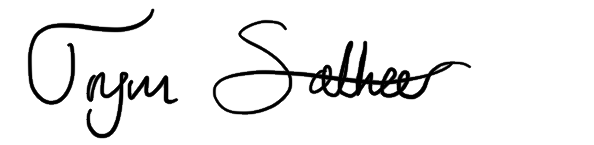
\includegraphics[height=1cm]{frontmatter/TS_Signature.png}\par
            \vspace{0.2cm}  % Reduced from 0.3cm
            {\color{ntnu-purple}\textit{Physics and Mathematics}}\par
        \end{flushleft}
    \end{minipage}
    \hfill
    \begin{minipage}{0.35\textwidth}
        \begin{flushright}
            \large
            {\color{ntnu-blue}\textbf{Semester}}\par
            \vspace{0.15cm}  % Reduced from 0.2cm
            Spring 2025\par
            6th semester
        \end{flushright}
    \end{minipage}
    \vfill  % This automatically fills available space
    {\sffamily Department of Mathematical Sciences} \par
    {\color{ntnu-blue}\sffamily Norwegian University of Science and Technology}
\end{titlepage}


\tableofcontents

\section{Overview}

\begin{description}[style=nextline]

    \item[Maximum-Norm Error Bounds:]
          Analyzing global error in the $\infty$-norm (max norm) for difference schemes. Using stability (e.g. via a discrete maximum principle or matrix norms) plus consistency to bound the error by a constant times the mesh step power.

    \item[Discrete Maximum Principle (DMP):]
          A property of certain finite difference operators ensuring that a discrete solution cannot attain new extrema in the interior. Often used to prove stability in max norm for elliptic problems (requiring coefficients like $\beta \geq \alpha + \gamma$).

    \item[Von Neumann Stability Analysis:]
          Fourier (modal) analysis for time-dependent schemes. One assumes a solution ansatz $U^n_m = \xi^n e^{i\beta x_m}$, derives the amplification factor $\xi$, and imposes $|\xi| \le 1$ to get stability criteria (e.g. CFL conditions).

    \item[Weak Form \& Galerkin FEM:]
          Reformulating PDEs into weak (variational) form by integration by parts, then approximating in a finite-dimensional subspace. Leads to the Galerkin equations $A\mathbf{u}=\mathbf{F}$, where $A$ is symmetric positive-definite (SPD) and arises from the bilinear form (stiffness matrix).

    \item[Finite Element Stiffness Matrix Assembly:]
          Computing $A_{ij}=\int \nabla \phi_i \cdot \nabla \phi_jdx$ (in 1D, $A_{ij}=\int_0^1 \phi'_i(x)\phi'_j(x)dx$) element by element and assembling globally. For 1D linear elements, this yields the familiar tridiagonal matrix ($2$ on diagonal, $-1$ off-diagonal) scaled by the element length.

    \item[Iterative Solvers (Jacobi \& CG):]
          Methods to solve the linear systems from discretization. Jacobi iteration updates each point from neighbors and converges under conditions like strict diagonal dominance (spectral radius $<1$). Conjugate Gradient (CG) is used for SPD systems; it converges in at most $n$ steps, with error reduction per step bounded by $(\sqrt{\kappa}-1)/(\sqrt{\kappa}+1)$ where $\kappa$ is $A$'s condition number.
\end{description}

\section{Detailed Topic Guide}

\subsection{Maximum-Norm Error Bounds}
\paragraph{Typical exam questions}
\begin{itemize}
    \item \enquote{Prove that the scheme is $O(h^2)$ convergent in the max norm.} Given a boundary-value problem and a second-order finite difference scheme, show that the maximum error $\max_m |e_m|$ is bounded by a constant times $h^2$.
    \item \enquote{Show the approximation is max-norm stable.} For example, proving $|U|_{\infty} \le C|f|_{\infty}$ for the discrete solution of $L_h U = f$ (a form of stability).
\end{itemize}

\paragraph{Worked outline}
To bound the error in $\infty$-norm, one uses consistency + stability $\Rightarrow$ convergence. 

\begin{description}[style=nextline]
    \item[Consistency:] First, perform a local truncation error expansion to verify the scheme is $p$th-order consistent (e.g. truncation $\tau_i = O(h^2)$). 
    \item[Stability:] Next, establish stability in max norm: for a linear system $A U = F$ derived from the scheme, stability means $|A^{-1}|_{\infty} \le C$ independent of $h$. 
    Often this is shown via a DMP argument or by proving $A^{-1}$ has nonnegative entries summing to $\le C$. 
    \item[Convergence:] Finally, by combining these, one concludes $|e|_{\infty} = |A^{-1}\tau|_{\infty} \le |A^{-1}|_{\infty}|\tau|_{\infty} \le C\cdot O(h^p)$, hence $\max|u(x_i)-U_i|=O(h^p)$. 
\end{description}

For example in a 1D elliptic BVP with a 5-point Laplacian, one can construct a barrier function to show stability (see DMP below) and use $\tau=O(h^2)$ to get $O(h^2)$ convergence. 
The key is demonstrating a uniform max-norm bound on the inverse difference operator.
\footnote{Owren (2017): Chapter 6, pp. ~76--78 -- Stability and global error analysis for elliptic difference schemes.}

\paragraph{Pitfalls}
\begin{itemize}
    \item \textbf{Mixing up local vs global error:} Don't assume $O(h^2)$ truncation implies $O(h^2)$ solution error without a stability argument. Remember that convergence requires both consistency and stability (Lax equivalence theorem).
    \item \textbf{Neglecting boundary effects:} For certain schemes, truncation error at or near boundaries might drop order. A common mistake is to ignore that the global error is often limited by the lowest-order accuracy in the domain (e.g. first-order at boundary can make overall $|e|_{\infty}=O(h)$). Be cautious and, if needed, refine the mesh or use a correction to maintain overall order.
    \item \textbf{Insufficient stability reasoning:} Merely citing that the matrix $A$ is invertible or SPD is not a full stability proof. You must show a bound like $|A^{-1}| \le C$ explicitly (often via DMP or matrix norm estimates). A frequent trap is to assert stability without showing how the discrete Green's function is bounded. Always argue why no large growth of error can occur.
\end{itemize}

\clearpage

\subsection{Discrete Maximum Principle (DMP)}
\paragraph{Typical exam questions}
\begin{itemize}
    \item \enquote{Prove that $-L_h$ has positive coefficients and satisfies a discrete maximum principle.} For instance, given a difference operator $L_h u_i = \alpha u_{i-1} - \beta u_i + \gamma u_{i+1}$ with $\alpha,\beta,\gamma>0$ and $\beta \ge \alpha+\gamma$, show that if $L_h v \le 0$ for interior points and $v$ is zero on the boundary, then $v_i \le 0$ for all interior $i$.
    \item \enquote{Show that the scheme preserves the maximum principle.} E.g., for a 2D Laplace equation discretization, prove that if $f_{ij}\ge0$ (or $\le0$) and $u$ satisfies $L_h u = f$ with zero boundary values, then $u_{ij}$ attains its extrema on the boundary (non-positive inside in this case).
\end{itemize}

\paragraph{Worked outline}
The DMP proof is typically by contradiction.

Assume the discrete solution attains a positive interior maximum at node $m$ (so $v_m = \max_n v_n > 0$ and $v_m \ge v_{m\pm1}$).

For a 1D three-point stencil under the given conditions,
$$
-L_h v_m = \alpha v_{m-1} - \beta v_m + \gamma v_{m+1} \le 0$$

plugging in the extremum gives

$$-\beta v_m + \alpha v_{m-1} + \gamma v_{m+1} \le 0.$$

But at $m$, $v_{m-1},v_{m+1}\le v_m$, so this implies

$$-\beta v_m + (\alpha+\gamma) v_m \le 0 \Rightarrow (\alpha+\gamma - \beta)v_m \le 0. \quad \text{with} \quad \beta \ge \alpha+\gamma$$,

this forces $v_m \le 0$, contradicting $v_m>0$.

Hence no interior node can exceed the boundary maximum.  A similar argument holds for a negative minimum.


In higher dimensions or more complex stencils, one uses an induction on neighbors or graph argument but the essence is the same: if $-L_h$ has all positive off-diagonals and each diagonal $\beta_{ii} \ge \sum_{j\neq i}\beta_{ij}$, then $L_h v \le 0$ forces $v$'s max to occur on the boundary (a property of M-matrices). This principle is then used to show stability: taking $v = e$ (error) or $v = e \pm \phi$ for some auxiliary $\phi$, one derives $\max |e|$ bounded by boundary values or forcing term. For example, in 2024 Exam Problem 1, after showing $-L_h$ positive, one had to prove DMP and then conclude max-norm stability by applying it to the error with a suitable supersolution.\footnote{Owren (2017): pp. 75--78 -- Definition and use of the discrete max principle for elliptic difference equations (implied by M-matrix conditions).}

\paragraph{Pitfalls}
\begin{itemize}
    \item \textbf{Coefficient conditions:} Forgetting the precise conditions under which DMP holds. Counterexample: If the scheme is not diagonally dominant (e.g. $\beta < \alpha+\gamma$), the DMP conclusion may fail. Always state and check that $-L_h$ yields $\beta_{ii}\ge \sum_{j\neq i}\beta_{ij}$ and off-diagonals $\ge0$ (no negative connections), otherwise the principle can't be applied.
    \item \textbf{Boundary values in DMP:} A common oversight is mishandling nonzero Dirichlet or Neumann boundary conditions. The simple form of DMP assumes homogeneous Dirichlet BC (boundary $v=0$). If $v$ is nonzero on the boundary, the conclusion should be $\max_{all} v = \max(\max_{\text{boundary}}v, 0)$. Adjust the statement accordingly or consider applying DMP to $v - B$ where $B$ is an extension of boundary values into the domain.
    \item \textbf{Sign convention errors:} Ensure the inequality direction is correct. DMP proofs can be done with $L_h v \ge 0$ or $\le0$; be consistent. If you assume $L_h v \le 0$ (as is common when $L_h$ is the Laplace operator approximation), you conclude $v$ has no positive interior max. If the inequality is flipped, the conclusion flips to no negative interior min. Keep track of these details to avoid losing marks on logical accuracy.
\end{itemize}

\clearpage
\subsection{Von Neumann Analysis}

\paragraph{Typical exam questions}
\begin{itemize}
    \item \enquote{Perform a von Neumann stability analysis of the scheme and find the CFL condition.}For example, given an explicit scheme for $u_t + au_x = 0$ or $u_t = \nu u_{xx}$, determine for what time-step $k$ relative to mesh $h$ the method is stable (often yielding $ak/h \le 1$ or $\nu k/h^2 \le 1/2$, etc.).
    \item \enquote{Is the scheme unconditionally stable or conditionally stable? Justify by Fourier analysis.} E.g., backward Euler for diffusion is unconditionally stable, which can be confirmed by showing the amplification factor $|\xi| = 1/(1+2r\sin^2(\frac{\beta h}{2})) < 1$ for all $r=k/h^2>0$. Conversely, for an explicit scheme, find the condition on $r$ so that $|\xi| \le 1$ for all Fourier modes $\beta$.
\end{itemize}

\paragraph{Worked outline}
Procedure: Assume a solution of the form $U^n_m = \zeta^n e^{i\beta x_m}$ (where $x_m = m h$). Substitute this into the homogeneous linear difference scheme. This yields a characteristic equation for the amplification factor $\zeta$. For a two-level scheme, one typically gets a relation $\zeta = G(\beta; \mu)$, where $\mu$ is the Courant number or similar parameter (e.g. $\mu=ak/h$ for advection, or $r=\nu k/h^2$ for diffusion). The Von Neumann criterion demands $|\zeta(\beta)| \le 1$ for all Fourier modes $\beta$ in $[-\pi/h,\pi/h]$.

In practice, one often checks the worst-case $\beta$ (like $\beta h = \pi$ for oscillatory mode). Example: For the FTCS scheme of the heat equation $u_t=\nu u_{xx}$ (forward time, central space), one finds $\zeta = 1 - 4r\sin^2(\frac{\beta h}{2})$. The stability requirement $|\zeta| \le 1$ for all $\beta$ leads to $|1 - 4r\sin^2(\theta)| \le 1$ $\forall \theta$, which simplifies to $4r\sin^2\theta \le 2$ (worst at $\sin^2\theta=1$), giving $r=\nu k/h^2 \le 1/2$. This is the familiar CFL condition $\nu k \le \frac{1}{2}h^2$.

Another example: for upwind advection, $\zeta = 1 - \mu(1-e^{-i\beta h})$; requiring $|\zeta| \le 1$ yields $\mu \le 1$ (CFL $a k \le h$). If the scheme is unconditionally stable (e.g. Crank--Nicolson or backward Euler for diffusion), the analysis will show $|\zeta| \le 1$ for all $r>0$ (often straightforward since $\zeta = \frac{1}{1+4r\sin^2(\frac{\beta h}{2})}$ in backward Euler, which is always $<1$).

Present the result as a clear condition (like $k \le h/|a|$ or $k \le h^2/(2\nu)$). If asked for amplification factor, give $\zeta(\beta)$ explicitly; if asked for stability, provide the derived inequality and conclude whether it's conditional or unconditional. Always mention the worst-case mode that dictates the condition (usually the highest frequency $\beta h = \pi$). The von Neumann criterion can be phrased as: the scheme is stable iff $\exists \mu \ge 0$ such that $|\zeta| \le 1 + \mu k$ (Lax's criterion) which essentially reduces to $|\zeta| \le 1$ as $k \to 0$.\footnote{Owren (2017): §5.9, pp. 60--62 -- Von Neumann's stability criterion and examples.}

\paragraph{Pitfalls}
\begin{itemize}
    \item \textbf{Complex roots and damping:} If $\zeta$ is complex, you must check $|\zeta| \le 1$, not $\Re(\zeta) \le 1$. Students sometimes erroneously set real and imaginary parts $\le 1$ separately. Use $|\zeta|^2 = \zeta \overline{\zeta}$ to include both amplitude and phase. For instance, with diffusion-advection combinations, $\zeta$ can be complex, so compute $|\zeta|^2$ properly.
    \item \textbf{Ignoring worst-case $\beta$:} It's a common mistake to plug in $\beta=0$ and conclude stability (since $\zeta(0)=1$ often). The most restrictive case is typically $\beta h = \pi$ (mode oscillating as +1, -1, +1, -1), so always evaluate at the highest frequency. If the scheme has multiple modes (multi-step schemes), consider all characteristic equation roots.
    \item \textbf{CFL vs absolute stability:} Don't confuse von Neumann CFL conditions with other stability notions. For linear constant-coefficient PDEs they coincide, but if the exam problem has variable coefficients or nonlinear terms, von Neumann analysis is only a necessary condition. So, state clearly that you assume constant coefficients or small perturbation analysis. If the coefficients are time- or space-dependent (as in some exam tasks), you might use a ``frozen coefficient'' analysis and mention that the CFL condition should hold for the maximum characteristic speed in the domain.
\end{itemize}

\clearpage

\subsection{Weak Form \& Galerkin FEM}
\paragraph{Typical exam questions}
\begin{itemize}
    \item Derive the weak/variatonal form of the given BVP. For example, start with $- (p(x)u')' + q(x)u = f(x)$ on $[a,b]$ with $u(a)=u(b)=0$, and derive $\int_a^b pu'v' + quv = \int_a^b fv$ for all test functions $v$.
    \item State the Galerkin method and set up the linear system. Often following the above, choose piecewise linear basis functions on a mesh and deduce that $u_h(x)=\sum_j U_j \phi_j(x)$ leads to the linear system $A\mathbf{U}=\mathbf{F}$ with $A_{ij}=\int p\phi'_i\phi'_j + q\phi_i\phi_jdx$ and $F_i=\int f\phi_idx$.
    \item Explain why $A$ is symmetric positive-definite (SPD). Usually, argue that $A_{ij} = a(\phi_j,\phi_i)$ for some bilinear form $a(\cdot,\cdot)$, hence $A=A^T$; and for PD, $a(v,v)=0$ implies $v=0$ in $V$ (by coercivity of the underlying PDE operator).
\end{itemize}

\paragraph{Worked outline}
\begin{enumerate}
    \item Start by multiplying the PDE by a test function $v(x)$ and integrating over the domain. 
    \item For a second-order ODE/PDE, integration by parts is performed to shift derivatives from $u$ onto $v$. 
    In a classic example, $-u''(x)=f(x)$ on $(0,1)$ with $u(0)=u(1)=0$: 
    multiply by $v$ and integrate, 
    $$\int_0^1 -u''(x)v(x)dx = \int_0^1 f(x)v(x)dx.$$

    \item Integrate the left by parts: 
    $$\int_0^1 -u'' vdx = \int_0^1 u' v'dx - [u'v]_0^1.$$ 
    The boundary term vanishes because $v(0)=v(1)=0$ for admissible test functions (they must satisfy the homogeneous BC). 
    \item This yields the weak form: 
    \begin{align*}
    \text{find} \; u \in V \;  \text{s.t} \int_0^1 u' v'dx = \int_0^1 f vdx, \; \forall \, v\in V \; (\subset V=H^1_0(0,1)).
    \end{align*}
    Where the Sobolev space $H^1_0(0,1) = \{u \in H^1(0,1) : u(0)=u(1)=0\}$ is the space of piecewise linear functions vanishing at the boundary.
    \item Next, apply the \textbf{Galerkin method}: restrict to a finite-dimensional subspace $V_h \subset V$ spanned by basis functions $\{\phi_j(x)\}_{j=0}^M$, typically hat functions at mesh nodes:
    \begin{align*}
        \phi_j(x) = \begin{cases}
            1 - |x-x_j|/h & \text{if } x \in [x_j-h,x_j+h] \\
            0 & \text{otherwise}
        \end{cases}\\
        &=
        \begin{cases}
            \frac{x-x_{j-1}}{x_j-x_{j-1}} & \text{if } x \in [x_{j-1},x_j] \\
            \frac{x_{j+1}-x}{x_{j+1}-x_j} & \text{if } x \in [x_j,x_{j+1}] \\
            0 & \text{otherwise}
        \end{cases}
        \tag{(hat function)}
    \end{align*}
    \item Assume approximate solution $u_h(x)=\sum_{j} U_j \phi_j(x).$
    Plugging $u_h$ into the weak form and choosing $v=\phi_i$ in turn yields the linear system: 
    $$\sum_j U_j \int_0^1 \phi'_j \phi'_idx = \int_0^1 f\phi_idx \quad \forall i=0,\ldots,M.$$
    In matrix form, 
    $$A\mathbf{U} = \mathbf{F}$$ 
    with entries 
    $$A_{ij}=\int \phi'_i \phi'_j, \quad F_i=\int f\phi_i.$$
    \item The matrix $A$ is symmetric since $A_{ij} = \int \phi'_i \phi'_j = \int \phi'_j \phi'_i = A_{ji}$ (bilinear form symmetry).
\end{enumerate}

Many exams simply expect you to note that $A_{ij}=a(\phi_i,\phi_j)$ for the symmetric bilinear form $a(u,v)=\int pu'v' + quv$, so $A$ is symmetric, and $a(v,v)=0$ implies $v=0$ due to the PDE's coercivity, hence PD.

Finally, note any specifics: e.g., if non-homogeneous BCs, one might incorporate them by a change of variable $u_h = R + w_h$ (lifting the BCs) as seen in some exams (like 2018 Exam Problem 1a). But typically, weak form derivations assume homogeneous BC to simplify.

In summary, the Galerkin procedure involves:
\begin{enumerate}[label=(\roman{*})]
    \item derive weak form,
    \item choose $V_h$ and basis,
    \item assemble $A$ and $\mathbf{F}$,
    \item solve $A\mathbf{U}=\mathbf{F}$.
\end{enumerate}

These steps are explicitly highlighted in Curry's notes.\footnote{Curry (2018): §2.1, pp. 3--5 -- Derivation of weak form for a 2nd-order ODE; Galerkin method steps.}
\paragraph{Pitfalls}
\begin{itemize}
    \item \textbf{Omitting boundary conditions in $V$:} A very common mistake is failing to enforce homogeneous Dirichlet conditions in the test/solution space. If $v$ doesn't vanish on the boundary, the integrated-by-parts formula will have extra boundary terms -- the derived weak form would then be incorrect. Always specify $V$ as, e.g., $H^1_0$ (functions vanishing on Dirichlet boundaries) so that those terms drop out.
    \item \textbf{Sign errors in integration by parts:} Keep track of the minus sign when moving the derivative: $\int -u''v = \int u'v'$, since $- \int u''v = -[u'v]_a^b + \int u'v'$. It's easy to lose a minus sign or a boundary term. Double-check by differentiating the weak form back to the strong form if possible.
    \item \textbf{Misidentifying test vs trial functions:} Remember, the weak form $\int a(u,v) = \int f v$ must hold for all $v$ in $V$. In practice, when assembling, we set $v=\phi_i$ to get the $i$th equation. Don't think of ``$v$'' as a single specific function; treat it as an arbitrary test function. This ensures you get a linear system that holds for each basis function weight (hence for all $v$).
    \item \textbf{Matrix assembly confusion:} Some assume the Galerkin equations magically appear without integration. In fact, you derive $A_{ij} = \int (\text{terms of }\phi_i,\phi_j)$ from the weak form. Avoid plugging trial functions into the strong form directly -- that leads to a collocation or least-squares method, not Galerkin. Stick to the variational form for deriving $A$ and $F$.
\end{itemize}

\subsection{Finite Element Stiffness Matrix Assembly}
\paragraph{Typical exam questions}
\begin{itemize}
    \item \enquote{Compute the element stiffness matrix for [a given element].}
     For instance, in a 2D Poisson problem with quadratic basis on a reference square (Exam 2016), find the $4\times4$ element matrix 
     $$A^K_{ij} = \iint_K (\nabla \phi_i \cdot \nabla \phi_j)dxdy.$$
    \item \enquote{Assemble the global matrix.}
    E.g., given a simple mesh or numbering, add up element contributions to form the final $A$. A common task: confirm that for linear elements in 1D, assembling yields the tridiagonal matrix with $2$ on the diagonal and $-1$ on off-diagonals (scaled by material coefficients and element length) -- essentially the discrete second-derivative matrix.
    \item \enquote{Discuss the structure of $A$.}
    Is it symmetric? Banded? What is the bandwidth? Is it an M-matrix? Many exam questions (2013, 2018) asked whether $A$ is tridiagonal, SPD, etc., expecting reasoning from the element connectivity and properties of the bilinear form.
\end{itemize}

\paragraph{Worked outline}
For each finite element element $K$, we compute the local stiffness matrix $A^K$ by integrating basis function gradients over that element. 

For example, in 1D with linear basis on interval $[x_k,x_{k+1}]$, there are two local shape functions $\phi_k,\phi_{k+1}$ that are 1 at one node and 0 at the other. Their derivatives on that element are constants: $\phi'_k = -1/h$, $\phi'_{k+1}=1/h$.

Thus the element matrix is:
\begin{align*}
    A^K = \begin{pmatrix}
        \int_K \phi'_k \phi'_kdx    & \int_K \phi'_k \phi'_{k+1}dx    \\[6pt]
        \int_K \phi'_{k+1}\phi'_kdx & \int_K \phi'_{k+1}\phi'_{k+1}dx
    \end{pmatrix} = \int_{x_k}^{x_{k+1}}\frac{1}{h^2} \begin{pmatrix}1 & -1\\ -1 & 1\end{pmatrix} dx = \frac{1}{h}\begin{pmatrix}1 & -1\\ -1 & 1\end{pmatrix},
\end{align*}

since $\int_{x_k}^{x_{k+1}} dx = h$. 

In general, for linear elements the $2\times2$ local matrix always looks like

$$
\frac{p(x_k)}{h}\begin{pmatrix}1&-1\\-1&1\end{pmatrix}
$$

if $p(x)$ is constant on $K$ (or replace $1/h$ by $\int_K p/h$ if variable).

Higher-order elements yield larger local matrices (e.g. $4\times4$ for a biquadratic square element as in 2016 exam, which require integrating quadratic polynomials -- one can use area coordinates or reference element integration formulas).

\textbf{Global assembly:} The global matrix $A$ is initially all zeros. For each element $K$ connecting global nodes $(i,j)$, add the entries of $A^K$ into the global $A$ at rows/cols $(i,j)$. 
In 1D, each element connects node $k$ and $k+1$, so each local matrix adds into the $2\times2$ block of $A$ at indices $(k,k), (k,k+1), (k+1,k), (k+1,k+1)$. After assembling all $M$ intervals, the resulting $A$ has the pattern:
$$ A = \frac{1}{h}\begin{pmatrix}
        1      & -1     & 0      & \cdots & 0      \\
        -1     & 2      & -1     & \cdots & 0      \\
        0      & -1     & 2      & -1     & \ddots \\
        \vdots &        & \ddots & \ddots & -1     \\
        0      & \cdots & 0      & -1     & 1
    \end{pmatrix}, $$
for homogeneous Dirichlet ends. 
This is exactly the matrix of the second difference operator.

In exams, you might only need to assemble a small example by hand. 
For instance, if $M=2$ (three nodes), assembling the two element matrices yields a $3\times3$ $A$ that you can write out. 
Always ensure to account for shared nodes: interior nodes accumulate contributions from two elements, hence the $2$ on the diagonal after summing two $1$'s. 

For the \textbf{load vector} $F$, similarly compute local $F^K_i = \int_K f\phi_idx$ and add to global $F$. Often, if $f(x)$ is simple, you can do these integrals (e.g. for linear $\phi$, $F^K = \frac{h}{2}(f(x_k), f(x_{k+1}))^T$ if using midpoint or linear interpolation approximations).

\textbf{Matrix properties:} From assembly logic, each interior node typically connects to itself and a few neighbors. Thus $A$ is \textbf{sparse} and often banded (bandwidth corresponds to max nodes per element). In 1D, bandwidth is 1 (tridiagonal). In a 2D grid with linear elements, bandwidth is larger but still on the order of $\sqrt{N}$. Exams often expect recognition that $A$ is symmetric (follows from $A_{ij}=A_{ji}$ by construction) and usually \textbf{M-matrix}-like (positive diagonal, negative off-diagonals for diffusion problems).

For example, in 2013 Problem 1b, after deriving the FEM system, one had to comment: Is $A$ symmetric? (Yes, $A=A^T$), Is it positive definite? (Yes, weak form is coercive), Is it tridiagonal? (In 1D, yes; in 2D, it's banded but not strictly tri-). By assembling or simply by knowing the support of basis functions (each linear basis overlaps only with its immediate neighbors), you can answer such questions confidently.\footnote{Curry (2018): §2.1--2.2, pp. 5--7 -- Definition of stiffness matrix and load vector; elementwise assembly process.}

\paragraph{Pitfalls}
\begin{itemize}
    \item \textbf{Assembly indexing errors:} A common mistake is adding local contributions to the wrong global entries. Always keep track of the global node numbering of each element. Drawing a small diagram of nodes vs element can help prevent misplacement of terms.
    \item \textbf{Omitting elementwise integration:} Some students try to write down the global matrix by intuition without computing any integrals. While pattern recognition is good, you should derive at least one local integral to justify the entries (especially if coefficients are not constant). For instance, if $p(x)$ varies, $A_{ii} = \int (p\phi'_i\phi'_i)$ might not equal $2p/h$ but rather an average. Avoid guessing -- do the integral or at least set it up.
    \item \textbf{Boundary conditions in assembly:} Remember to apply boundary conditions to $A$ and $F$. For homogeneous Dirichlet, the first and last basis functions might be omitted entirely (if $u_0=u_M=0$ are known, then $U_0,U_M$ are not unknowns -- thus $A$ effectively is smaller). If you include them, you must incorporate the BC by modifying $A$ or $F$ (e.g. subtracting known terms). Forgetting this leads to an inconsistent system.
    \item \textbf{Confusing FD and FE matrices:} The structure may look similar to finite difference, but the derivation is different. Don't mix up stencil intuition with assembly. For example, a Robin boundary condition in FEM adds a term in $A_{nn}$ and $F_n$ (from the boundary integral), whereas in FD one might tweak the last equation differently. Be precise with FEM: incorporate boundary integrals for natural BCs, and enforce essential BCs by adjusting the linear system (big penalty or modification method).
\end{itemize}

\subsection{Iterative Solvers (Jacobi \& Conjugate Gradient)}
\paragraph{Typical exam questions}
\begin{itemize}
    \item \enquote{Will the Jacobi iteration converge for this system? For which parameter values?} e.g., given a $3\times3$ matrix $A(\alpha,\beta)$, determine for what $\alpha,\beta$ the spectral radius $\rho(D^{-1}R)<1$. In 2018 Exam (Problem 4b), students solved a specific $3\times3$ system, finding that Jacobi converges if $\alpha > |\beta|$ (ensuring diagonal dominance).
    \item \enquote{Show that the Jacobi method converges for any SPD $2\times2$ matrix, but can diverge for some SPD $n\times n$.} (This type of question appeared in 2015/2016 exams.) It tests understanding that SPD is not a sufficient convergence condition for Jacobi in general -- counterexamples exist when off-diagonals are large despite SPD.
    \item \enquote{Estimate the number of CG iterations needed to reach tolerance $\varepsilon$.} For example, \textit{``Given eigenvalues of $A$ lie in $[a,b]$, how many iterations $K$ are needed for $\frac{\|e_K\|_A}{\|e_0\|_A}\le \varepsilon$?''} -- using the CG convergence bound involving $\sqrt{b/a}$ (condition number). An exam might give specific $a,b$ or ask you to use an approximate ratio from an eigenvalue formula of $A$.
\end{itemize}

\paragraph{Worked outline}
\textbf{Jacobi Method:} We split $A = D - R$ where $D=\operatorname{diag}(A)$ and $R = D - A$ (so $R$ contains off-diagonals). The Jacobi iteration is:
\[ x^{(k+1)} = D^{-1}(R x^{(k)} + b), \]
or component-wise $x_i^{(k+1)} = \frac{1}{a_{ii}}\sum_{j\neq i} a_{ij}x_j^{(k)} + \frac{1}{a_{ii}}b_i$. The iteration matrix is $M = D^{-1}R = I - D^{-1}A$. Jacobi converges if and only if $\rho(M)<1$. A sufficient (though not necessary) condition is strict diagonal dominance: $|a_{ii}| > \sum_{j\neq i}|a_{ij}|$ for all $i$. In that case, by the Gershgorin circle theorem, $\rho(M)<1$ holds, so convergence is guaranteed.

For example, for the 1D Poisson matrix ($2$ on diag, $-1$ off), Jacobi's $\rho = |\frac{-1}{2}| = 0.5 < 1$ so it converges. In an exam scenario, one might take a given $A$, compute $M = D^{-1}R$, and find its eigenvalues or spectral radius. Often, symmetry plus a diagonal dominance argument suffices: In 2018 (Problem 4b), $A=\begin{pmatrix}\alpha & \beta &0\\ \beta&\alpha&\beta\\0&\beta&\alpha\end{pmatrix}$ -- one can show $\rho(M)=|\frac{\beta}{\alpha}|$ for large systems, hence require $|\beta|<\alpha$.

Another approach: for SPD $A$, Jacobi converges \textit{if} $A$ is also diagonally dominant or symmetric \textit{and} weakly diagonally dominant with positive diagonal entries (which SPD ensures) -- but as a counterexample, a dense SPD matrix can break Jacobi (2015 exam exhibited $A=I+\kappa E$ where $E$ has all entries 1; $A$ is SPD but Jacobi diverges because off-diagonals are too large, $\rho(M)>1$). So the takeaway is: check diagonal dominance or find $\rho(M)$ explicitly for the matrix at hand.

\textbf{Conjugate Gradient (CG):} CG is the method of choice for large SPD systems. It produces a sequence of approximations $x^{(k)}$ that minimizes the $A$-norm of the error over the Krylov subspace. The notable convergence result:
\[ \frac{\|e_{k}\|_A}{\|e_0\|_A} \le 2\left(\frac{\sqrt{\kappa}-1}{\sqrt{\kappa}+1}\right)^k, \]
where $\|v\|_A := \sqrt{v^T A v}$ and $\kappa = \frac{\lambda_{\max}(A)}{\lambda_{\min}(A)}$. In practice, this means the error drops \textit{at least} at a rate of roughly $\left(\frac{\sqrt{\kappa}-1}{\sqrt{\kappa}+1}\right)$ per iteration. For large $\kappa$, this is slow; preconditioning is used to reduce $\kappa$.

In exam problems, you may be given an estimate of eigenvalue bounds. For instance, if $A$ comes from a 2D Poisson with mesh size $h$, one might use known eigenvalue estimates (like $\lambda_{\min}\approx C h^2$, $\lambda_{\max}\approx C'$, so $\sqrt{\kappa}\sim 1/h$). Then plugging numbers: say $\kappa \approx 10^4$, then $(\sqrt{\kappa}-1)/(\sqrt{\kappa}+1)\approx (100-1)/(100+1)\approx 0.9802$. To get a factor $\varepsilon=10^{-7}$, one solves $0.9802^K \approx 10^{-7}$ giving $K \approx \frac{\ln(10^{-7}/2)}{\ln(0.9802)}$ (the ``2'' in front means we may loosely include a factor 2 as well). A simpler estimate: $K \gtrsim \frac{1}{2}\sqrt{\kappa}\ln(1/\varepsilon)$.

In 2013 Exam Problem 2b, for $M+1=100$ (so $M=99$ interior points in each dimension of a 2D grid) they found $\sqrt{\kappa}\approx \pi M/2 \approx 155$, and asked for $K$ with $\varepsilon=10^{-7}$ -- plugging in gives on the order of tens of iterations (the answer was around $K\approx 35$).

In summary, for Jacobi: state the iteration clearly and use either Gershgorin or known spectral radius formulas to decide convergence. For CG: quote the error bound formula and plug in the condition number or eigenvalues to get $K$. Also, note CG's nice property: if $A$ has only $m$ distinct eigenvalues, CG converges in at most $m$ steps (often much faster in practice than worst-case bound). This sometimes can be used if eigenstructure is given.

\paragraph{Pitfalls}
\begin{itemize}
    \item \textbf{Applying Jacobi to non-diag.-dominant SPD matrices:} 
    Students might wrongly assume \enquote{SPD implies Jacobi converges.}
    \medskip
    As highlighted in exams, SPD is \textit{not} sufficient -- e.g., the matrix with all off-diagonals $=0.5$ and diagonals $=1$ is SPD for certain sizes but Jacobi diverges. 
    \medskip
    The correct condition is $\rho(D^{-1}A - I)<1$. When in doubt, \textit{compute $\rho(M)$ or check a known criterion}. If given a numeric example, actually compute a few iterations or eigenvalues to verify convergence/divergence.
    \item \textbf{Forgetting prerequisites of CG:} CG only works for symmetric positive-definite $A$. A common error is discussing CG for a non-symmetric matrix or not noticing that a linear system isn't SPD (e.g. an unsymmetric advection-diffusion matrix -- one should mention using BiCG or GMRES in reality, but if asked about CG, likely $A$ was SPD). If an exam problem implicitly assumes SPD (as many do when referencing CG), ensure you mention symmetry and definiteness as justification for applying CG.
    \item \textbf{Mishandling the convergence bound:} The formula with $(\sqrt{\kappa}-1)/(\sqrt{\kappa}+1)$ can be tricky. Don't confuse $\kappa$ with $\sqrt{\kappa}$ in plugging values. Also, the factor 2 in front means after $k$ iterations, error $\le 2(\frac{\sqrt{\kappa}-1}{\sqrt{\kappa}+1})^k$ -- for large $k$ this 2 is negligible compared to the exponential decay, but for estimating \textit{exact} $K$ it might matter by a couple iterations. If unsure, you can drop the 2 for a rough estimate (as is often acceptable). Another pitfall: using $\kappa$ instead of $\sqrt{\kappa}$ in the fraction -- remember it's $\sqrt{\kappa}$ in that formula.
    \item \textbf{Stopping criterion vs error norm:} Exams might use the $A$-norm or energy norm for error. Be clear on what $\|e_K\|_A \le \varepsilon \|e_0\|_A$ means -- it's a relative error in the energy norm. Don't mix this up with, say, $\|r_k\|_2$ (residual norm) unless given a formula for that. If only eigenvalue bounds are given, stick to the $A$-norm convergence as above. If they ask for iterations to get $\|e_k\|_2/\|e_0\|_2 < \varepsilon$, you might note $\|e\|_2 \le \|e\|_A/\sqrt{\lambda_{\min}}$ to connect $A$-norm and 2-norm. Generally, clarify your norm assumptions to avoid confusion.
\end{itemize}

\section{Two-Hour Mock-Exam Checklist}

\begin{itemize}[leftmargin=*]
    \item \textbf{Derive finite difference formulas quickly:} Remember central difference for $u''(x) \approx \frac{u_{i-1}-2u_i+u_{i+1}}{h^2}$ (second order). For first derivative upwind vs central: central $\frac{u_{i+1}-u_{i-1}}{2h}$, upwind $\frac{u_i - u_{i-1}}{h}$ (first order). Re-derive if forgotten by Taylor expanding two points.

    \item \textbf{Max-norm error bound strategy:} Identify if the scheme matrix is an M-matrix (diag dom with non-neg off-diagonals). If yes, consider using DMP: \textit{Assume} interior error max and derive contradiction. Alternatively, recall $\|A^{-1}\|_{∞}$ for common matrices: for 1D Laplace $A$, $\|A^{-1}\|_{∞} = 1$ (each row of $A^{-1}$ sums to 1). Use $\|e\|_{∞} \le \|A^{-1}\|_{∞}\|\tau\|_{∞}$.

    \item \textbf{Discrete Maximum Principle conditions:} Check $a_{ii} \ge \sum_{j\ne i}a_{ij}$ and $a_{ij}\le 0$ (for $L_h u = f$ form) or equivalent. Write the inequality form and ensure you correctly identify the sign of $f$: e.g., to use DMP, typically write $L_h e = \tau$ and say for sufficiently small $h$, $\tau_i \le C h^p$ implies interior $e_i$ bounded by boundary $e$ plus $\tau$ term. Have a simple 1D proof outline ready (as done above).

    \item \textbf{Von Neumann analysis:} Write down the ansatz $U^n_m = \zeta^n e^{i\beta m h}$. Derive $\zeta$ formula carefully. Remember common results: for advection $u_t + a u_x=0$, FTBS (upwind) stability if $|a|\frac{k}{h} \le 1$; for diffusion $u_t=\nu u_{xx}$, FTCS stability if $\nu \frac{k}{h^2}\le \frac{1}{2}$. If stuck, test extreme modes: assume $u^n_m = (+1)^m$ and $(-1)^m$ to check growth.

    \item \textbf{Weak form essentials:} \textit{Integration by parts:} $\int (p u' v' + q u v) = \int f v$ after IBP for $p u''$. Boundary terms: $p u' v|_{a}^{b}$, which vanish if $v=0$ at boundaries. Always impose homogeneous BC in function space. If non-homog. BC: do $u = w + \tilde{u}$ trick (with $w$ satisfying BC). Know the standard weak form for Poisson: $\int \nabla u \cdot \nabla v = \int f v$.

    \item \textbf{Galerkin linear system:} Stiffness matrix formula: $A_{ij} = \int \nabla \phi_i \cdot \nabla \phi_j$ (plus $\int q\phi_i\phi_j$ if reaction term). Load: $F_i=\int f \phi_i$. For linear 1D hat functions: $A_{i,i}=2/h$, $A_{i,i+1}=A_{i+1,i}=-1/h$. Quickly recall the assembled matrix looks like (for $n$ interior nodes) $\frac{1}{h}\mathrm{tridiag}(-1,2,-1)$.

    \item \textbf{Matrix properties to mention:}
          \begin{itemize}
              \item \textbf{Symmetric:} Yes, if derived from variational form. From bilinear form $a(u,v)$, we get $A_{ij}=a(\phi_i,\phi_j)=a(\phi_j,\phi_i)=A_{ji}$.

              \item \textbf{Positive-definite:} Yes, for diffusion operators. Energy argument: $v^T A v = \int (\nabla v)^2 > 0$ for nonzero $v$.

              \item \textbf{Sparsity/bandwidth:} In 1D, bandwidth 1 (tridiagonal). Each row has at most 3 nonzeros since nodes only connect to nearest neighbors.

              \item \textbf{Block structure (2D):} For 2D problems, bandwidth is larger but still sparse. Typically 5 nonzeros per row for 5-point stencil, corresponding to center node plus its 4 neighbors.
          \end{itemize}
    \item \textbf{Jacobi iteration:}
          \begin{itemize}
              \item \emph{Formula:}
                    \[
                        x_i^{new} = \frac{1}{a_{ii}}\Big(b_i - \sum_{j\neq i}a_{ij}x_j^{old}\Big).
                    \]
              \item \emph{Convergence:}
                    require $\max_j |\frac{-a_{ij}}{a_{ii}}| < 1$ in some norm. If time is short, state diagonal dominance condition.
                    Remember Jacobi's spectral radius for simple cases: for $2\times2$ SPD $ \begin{pmatrix}a & b\\ b & a\end{pmatrix}$, $\rho(J) = |b|/a$.
          \end{itemize}
    \item \textbf{Gauss--Seidel:} (If mentioned) It's like Jacobi but sequential update, generally converges faster. Condition for GS is a bit weaker than Jacobi (still usually need diagonal dominance for guarantee). Not often asked in depth, but recall it if needed: GS iteration matrix eigenvalues are those of Jacobi squared, roughly.

    \item \textbf{Conjugate Gradient facts:} Only for SPD matrices. Each iteration minimizes error over a growing Krylov subspace. Know formula for error after $k$ steps (above). In practice, error drops rapidly: good rule, after \textasciitilde$n/2$ steps usually very small error for nice spectra. If asked, mention preconditioning improves $\kappa$.

    \item \textbf{CG iteration count estimate:} Use $\frac{\sqrt{\kappa}-1}{\sqrt{\kappa}+1}$. For rough estimates: if $\kappa = 10^4$, $\sqrt{\kappa}=100$, then error reduces by factor $\approx0.98$ each iteration, need on order of $\frac{1}{0.02}\ln(1/\varepsilon)$ iterations (for $\varepsilon=10^{-6}$, that's \textasciitilde$50\ln(10^6)\approx 50\cdot14 \approx 700$; but CG often outperforms worst-case). If eigenvalues cluster, convergence is faster. If time, mention these nuances but focus on using the bound formula correctly.

    \item \textbf{Final sanity checks:} Units and limits -- e.g., CFL condition $k \to 0$ or $h \to 0$ behavior should make sense (smaller $h$ demands smaller $k$ for explicit schemes). For FEM, if something seems off (like a stiffness matrix entry negative when it should be positive), recheck the integration. For iterative methods, if $\rho>1$, clearly state ``diverges.'' If $\rho<1$, maybe compute a numerical example iteration or two to illustrate convergence rate. And always link back to the theory: e.g., ``Since $|b/a|<1$, Jacobi will converge (spectral radius = $|b|/a$)''.
\end{itemize}

\section{Maximum-Norm Error Bounds}

\subsection{Step-by-Step Strategy}

\begin{enumerate}
    \item \textbf{Set up the error equation:} Let $u(x)$ be the exact solution and $U_m$ the numerical solution at grid point $x_m$. Define the error $e_m = U_m - u(x_m)$. Derive the error equation that $e_m$ satisfies by subtracting the discrete equation from the continuous one. For a linear problem, this often has the form $L_h e_m = \tau_m$, where $L_h$ is the discrete operator and $\tau_m$ is the local truncation error at $x_m$. Make sure to apply homogeneous boundary conditions to $e$ (e.g. $e=0$ at Dirichlet boundaries).

    \item \textbf{Estimate the truncation error:} Use Taylor expansions to bound $|\tau_m|$. For a $p$-th order scheme, one expects $|\tau_m| \leq Ch^p$ for some constant $C$. This gives a proxy for the error's magnitude. (For example, a second-order centered difference for $u''(x)$ yields $\tau_m = O(h^2)$ by Taylor's theorem.)

    \item \textbf{Identify stability properties:} Check if the coefficient matrix $A$ of the linear system $A \mathbf{U} = \mathbf{F}$ (or the operator $L_h$) has a structure that ensures max-norm stability. In practice, many elliptic finite difference matrices are M-matrices: they have positive diagonal entries, negative off-diagonals, and are strictly diagonally dominant. Such matrices yield a discrete maximum principle and a bounded inverse in $\ell_\infty$ norm. In other words, confirm that $-L_h$ has nonnegative coefficients (this is often true for self-adjoint second-order schemes).

    \item \textbf{Apply the discrete maximum principle or norm bound:} With the error equation $A e = \tau$, take the infinity-norm on both sides. One way is to use the matrix norm: $\|e\|_\infty = \|A^{-1}\tau\|_\infty \leq \|A^{-1}\|_\infty \|\tau\|_\infty$. If $A$ is an M-matrix, all entries of $A^{-1}$ are nonnegative and one can often show $\|A^{-1}\|_\infty$ is bounded by a modest constant (independent of $h$). Alternatively, use a discrete comparison argument: consider the maximum of $|e_m|$ over all grid points. If $|e_j|$ attains a strict maximum at an interior node $x_j$, then $L_h e_j = \tau_j$ together with the sign pattern of $L_h$ leads to a contradiction unless that maximum is controlled by the boundary or forcing. A common technique is to compare $e_m$ to solutions of $L_h w = \pm \|\tau\|_\infty$ (constant forcing) and use linearity to conclude $\|e\|_\infty \leq K\|\tau\|_\infty$ for some constant $K$ (often $K=1/2$ for typical 1D second-order problems).

    \item \textbf{Conclude the error bound:} Substitute the truncation error bound from step 2. You obtain an estimate like $\displaystyle \max_m |e_m| \leq KCh^p$. Thus, the global error in max-norm is $O(h^p)$, and you can confidently state the error bound (including the constant if needed). For example, one can prove for a 1D Poisson problem on $[a,b]$ that $\max_{m}|u(x_m)-U_m| \leq \frac{(b-a)^2}{2}\max_m|\tau_m|$, and hence with $|\tau_m|=O(h^2)$ one gets $\|e\|_\infty = O(h^2)$.
\end{enumerate}

\subsection{Common Slips to Avoid}

\begin{itemize}
    \item Don't assume the scheme is stable without checking the matrix structure. An error bound in $\ell_\infty$ norm typically requires the discrete operator to satisfy a maximum principle or a known norm bound.

    \item Avoid confusing the local truncation error $\tau_m$ with the global error $e_m$. You must propagate the local error through the system; a small $\tau_m$ does not automatically mean small $e_m$ without a stability argument.

    \item Remember to enforce boundary conditions on the error. If the exact solution satisfies the same BCs as the numerical solution, then $e=0$ at the boundaries, which is crucial for applying the maximum principle.

    \item Be careful with signs when forming the error equation. For example, if the continuous equation is $Lu=f$ and discrete is $L_h U = f$, the error equation is $L_h e = L_h(U - u) = L_h U - L_h u = f - L_h u$. But since $Lu=f$, the consistency error is $L_h u - Lu = \tau$. Keeping track of these terms is important for correctness.

    \item Don't lose track of the goal: after deriving $L_h e = \tau$, your objective is to show $\|e\|_\infty$ is bounded by a constant times $\|\tau\|_\infty$. Each step (matrix properties, maximum principle, etc.) should contribute to that end.
\end{itemize}

\subsection{Discrete Maximum Principle (DMP)}

\subsubsection{Step-by-Step Strategy}

\begin{enumerate}
    \item \textbf{Recognize the scenario for DMP:} The discrete maximum principle typically applies to linear steady-state problems (like Laplace or Poisson equations) discretized with schemes that produce an M-matrix. Write the interior grid equations in the canonical form:
          \begin{equation}
              a_{ii}U_i = \sum_{j \neq i} a_{ij}U_j + b_i
          \end{equation}

          for each interior node $i$. Here $a_{ii}>0$, and usually $a_{ij}\le 0$ for neighboring nodes $j$ (arising from second-order diffusion terms). Ensure any source term is denoted by $b_i$. For example, the 5-point Laplace FD stencil gives $4U_{i,j} - U_{i+1,j}-U_{i-1,j}-U_{i,j+1}-U_{i,j-1}=0$, which fits this pattern ($a_{ii}=4$, neighbors have coefficient $-1$).

    \item \textbf{Check boundary conditions:} DMP is about comparing interior and boundary values. For Dirichlet problems, the boundary values $U$ are known; often one assumes the maximum principle question is for the homogeneous case ($b_i=0$) or one considers a homogeneous comparison. If dealing with an inhomogeneous equation ($b_i \neq 0$), it helps to first subtract off a particular solution or otherwise transform the system so that you consider $L_h \tilde U = 0$ with modified boundary conditions. This might involve constructing a function $R(x)$ that satisfies the boundary conditions, letting $V = U - R$, so that $V$ satisfies a homogeneous BC problem.

    \item \textbf{Assume an interior extremum and derive a contradiction:} Suppose $U_k$ is an interior node where $U_k$ attains the maximum value among all nodes (interior + boundary). Let that maximum be $U_k = M$. Because $U_k \ge U_j$ for all neighbors $j$, and $a_{ij}\le 0$, we have $\sum_{j \ne k} a_{kj}U_j \le \sum_{j \ne k} a_{kj} M = M\sum_{j\ne k}a_{kj}$. The discrete equation at $k$ is $a_{kk} M = \sum_{j\ne k} a_{kj} U_j + b_k$. If $b_k=0$ (homogeneous case), then $a_{kk} M \le M \sum_{j\ne k}a_{kj}$. But since $a_{kk} = -\sum_{j\ne k} a_{kj}$ for typical self-adjoint schemes, this simplifies to $a_{kk} M \le -a_{kk} M$. This implies $(2a_{kk}) M \le 0$. Given $a_{kk}>0$, we get $M \le 0$. In other words, the interior maximum cannot be positive. By a symmetric argument, the interior minimum cannot be negative. Thus, any extremum of $U$ must occur on the boundary. This is the discrete maximum principle: $\max_{\text{interior}} U \le \max_{\text{boundary}} U$ and $\min_{\text{interior}} U \ge \min_{\text{boundary}} U$.

    \item \textbf{Handle inhomogeneous terms (if present):} If $b_i \neq 0$, the strict DMP as stated above doesn't directly apply because $L_h U = -b$ introduces a forcing. In that case, one strategy is to use a superposition argument. Solve or estimate two comparison problems: one with $L_h W = -\max_i b_i$ and one with $L_h Z = -\min_i b_i$. By linearity, $W_i$ and $Z_i$ will serve as upper and lower bounds for $U_i$. Another method is to augment $U$ by a specific solution $\phi$ of $L_h \phi = -b$, then $V = U - \phi$ satisfies $L_h V = 0$ with homogeneous boundary data, to which the earlier argument applies.

    \item \textbf{State the conclusion clearly:} Under the given conditions (typically, $a_{ii}>0$, $a_{ij}\le0$, diagonal dominance, etc.), no interior node can exceed the maximum boundary value or go below the minimum boundary value. This property ensures that if the boundary values of a discrete problem are all within a certain range, the interior will not "overshoot" that range. It's a powerful tool for ensuring stability of the solution, since it prevents non-physical oscillations or blow-up in the interior.
\end{enumerate}

\subsubsection{Common Slips to Avoid}

\begin{itemize}
    \item \textbf{Sign errors:} Ensure that you correctly identify the signs of coefficients. DMP usually requires something like $a_{kk} = \sum_{j\ne k}(-a_{kj})$, with $a_{kj} \le 0$ for neighbors. A common mistake is to carry a wrong sign through the inequality chain. Write out the inequality carefully when assuming $U_k$ is max.

    \item \textbf{Boundary vs. interior:} Don't apply the interior argument to boundary nodes. The principle is that the global maximum of $U$ occurs on the boundary; it doesn't say anything about boundary points themselves except that they could be the maxima. So avoid statements like "$U$ is constant" unless the boundary values themselves are constant.

    \item \textbf{Inhomogeneous confusion:} If there is a nonzero $b_i$, do not simply assert the DMP without modification. An interior maximum could occur if the forcing $b_i$ is positive at that point. Always address how the source term is handled.

    \item \textbf{Insufficient conditions:} Be cautious about the conditions for DMP. Irreducibility of the matrix or connectivity of the grid can matter. Also, strictly positive diagonal and non-positive off-diagonals are usually required. If the problem has variable coefficients, ensure they don't break the monotonicity.

    \item \textbf{Jumping to conclusions:} Don't just state the DMP result; show the steps (via contradiction). In exams, full credit usually requires clearly articulating why the interior value can't exceed the boundary value.
\end{itemize}

\section{Von Neumann Stability Analysis}

\subsection{Step-by-Step Strategy}

\begin{enumerate}
    \item \textbf{Write the update formula in a form suitable for Fourier analysis:} Take the difference scheme (typically for an initial-value PDE problem) and express it as an update equation. For example, a time-marching scheme might be written as $U^{n+1}_m = \sum_j \alpha_j U^n_{m+j}$ (explicit scheme) or $\sum_j \alpha_j U^{n+1}_{m+j} = \sum_j \beta_j U^n_{m+j}$ (for an implicit or multi-step scheme). Ensure the coefficients $\alpha_j, \beta_j$ are clearly identified. The scheme should have constant coefficients in space and time for Von Neumann analysis to apply.

    \item \textbf{Assume a Fourier mode solution:} Postulate a solution of the form $U^n_m = \xi^n e^{ikmh}$, where $k$ is a wavenumber and $h$ is the spatial step. Here $e^{ikmh}$ represents a complex sinusoidal mode on the grid, and $\xi$ is the amplification factor per time-step that we need to determine. Substitute this form into the update equation. Use the property that spatial shifts of the exponential are easy to handle: $U^n_{m+j} = \xi^n e^{ik(m+j)h} = \xi^n e^{ikmh} e^{ikjh}$. This will cause the exponentials to cancel out in the algebra, leaving a relationship for $\xi$.

    \item \textbf{Derive the amplification factor equation:} After substitution, divide out the common factor $e^{ikmh}\xi^n$ (which is nonzero). You will obtain an algebraic equation for $\xi$ in terms of $e^{ikh}$ (which is often denoted $z = e^{ikh}$ for convenience). For a simple example, the Forward Euler scheme for $u_t = \nu u_{xx}$ leads to: $\xi = 1 - 4\nu \frac{\Delta t}{h^2}\sin^2\frac{kh}{2}$ as the amplification factor for mode $e^{ikmh}$. In general, you get a symbol $G(kh)$ such that $\xi = G(kh)$. If the scheme is more complicated (like multi-step), you might get a polynomial in $\xi$ that you need to solve (e.g., for a two-step method, a quadratic equation in $\xi$ whose roots are the amplification factors).

    \item \textbf{Analyze $|\xi|$ for stability:} The scheme is (Von Neumann) stable if and only if all Fourier modes are non-amplifying, i.e., $|\xi(k)| \le 1$ for every wavenumber $k$ in the range of interest. Typically, $k$ ranges from $0$ up to the Nyquist frequency $\pi/h$ for grid spacing $h$. Now, take the expression for $G(kh)$ from step 3 and impose the stability condition $|G(kh)| \le 1$ for all $k$. This usually yields a constraint on the time-step $\Delta t$ relative to $h$ (for explicit schemes) or confirms unconditional stability (for implicit schemes). For instance, with the above heat equation example, $|1 - 4\nu \frac{\Delta t}{h^2}\sin^2(\frac{kh}{2})| \le 1$ for all $k$ leads to the requirement $0 \le 1 - 4\nu \frac{\Delta t}{h^2} \le 1$, which simplifies to $\nu \frac{\Delta t}{h^2} \le \frac{1}{2}$.

    \item \textbf{Find the worst-case (critical) scenario:} Often the most restrictive case is the highest frequency mode ($kh = \pi$, corresponding to alternating signs between grid points). Plugging that in typically gives the largest $|G|$. Solve for the threshold where $|G|=1$. For example, in the heat equation forward-Euler case, $kh = \pi$ gives $|1 - 4\nu \frac{\Delta t}{h^2}\sin^2(\pi/2)| = |1 - 4\nu \frac{\Delta t}{h^2}| \le 1$, leading to $4\nu \frac{\Delta t}{h^2} \le 2$. Thus $\Delta t \le \frac{1}{2}\frac{h^2}{\nu}$ is the stability condition (this is the famous CFL condition for the heat equation).

    \item \textbf{State the stability criterion and implications:} Conclude with a clear statement: e.g., "The scheme is stable for $\displaystyle \Delta t \le \frac{h^2}{2\nu}$." If the analysis shows $|\xi| < 1$ for all $k$ with no restriction, then the scheme is unconditionally stable. If $|\xi|\le 1$ only for $\Delta t$ equal to some value (e.g., exactly 1), the scheme is marginally stable or neutrally stable (errors don't grow, but also don't decay, often indicating the scheme is on the edge of stability). If any $|G|>1$ for some mode, the scheme is unstable (errors in those modes will amplify).

    \item \textbf{Verify the analysis assumptions:} Remember that Von Neumann analysis assumed linear constant-coefficient PDE and either an infinite or periodic domain (so that Fourier modes form a basis of solutions). In an exam answer, it's good to remark that this method gives a necessary condition for stability (and for linear constant coefficient problems, it's also sufficient). If the problem has boundaries or variable coefficients, von Neumann analysis is applied at least locally or as an estimate. But usually exam questions are set up so that full von Neumann analysis is valid (periodic BC or implicitly assuming large domain).
\end{enumerate}

\subsection{Common Slips to Avoid}

\begin{itemize}
    \item \textbf{Algebraic mistakes in substitution:} It's easy to drop a factor of $e^{ikh}$ or mis-handle the complex algebra. Write out a small example if unsure: for instance, check that a term like $U^n_{m+1}$ becomes $\xi^n e^{ik(m+1)h} = e^{ikh} \xi^n e^{ikmh}$. Keeping the exponent factor separate helps isolate the $\xi$ relation correctly.

    \item \textbf{Ignoring complex conjugates:} When assessing $|G| \le 1$, especially if $G$ is complex, ensure you consider $|G|^2 = G \overline{G}$ properly. Sometimes students solve $G=1$ or $G=-1$ instead of the magnitude. It's often easier to ensure the expression inside stays between -1 and 1 if it's real, or if $G = 1 + \mathrm{i}Y$, then require $|G|^2 = 1 + Y^2 \le 1$ which implies $Y=0$. Don't just take the real part.

    \item \textbf{Forgetting the "for all $k$" part:} A very common mistake is to find one particular mode (often $k= \pi/h$) and derive a condition, but neglect to check other modes. Always either argue that the worst case is at an endpoint of the spectrum or do a derivative test to find maxima of $|G(kh)|$. For many schemes, extreme $k$ (0 or Nyquist) are worst-case, but double-check the functional form of $|G|$.

    \item \textbf{Boundary conditions influence:} Von Neumann assumes an infinite or periodic domain to allow pure Fourier modes. In an exam solution, you can usually state this assumption. If the problem domain isn't periodic, strictly speaking von Neumann gives a necessary condition. Don't apply it blindly to a non-periodic problem without acknowledging this (examiners sometimes expect a note like "assuming the errors can be Fourier-expanded due to either periodic extension or large domain, we proceed with von Neumann analysis…").

    \item \textbf{Not simplifying the criterion:} After deriving an inequality, make sure to express the stability condition in simple terms (e.g. solve for $\Delta t$). Don't leave the answer as an implicit inequality involving $k$ and $h$. The whole point is to find a clear restriction like $\Delta t \le \text{(some function of $h$)}$. So isolate $\Delta t$ (or the parameter of interest) explicitly.

    \item \textbf{Distinguish stability vs. convergence:} Von Neumann analysis addresses stability. Sometimes students jump to saying "therefore the scheme is convergent if this holds." Technically, convergence requires consistency as well (Lax equivalence theorem). It's fine to mention convergence, but only after stating stability. In an exam though, usually the task is just to find the stability condition.
\end{itemize}

\section{Weak Form \& Galerkin Finite Element Method}

\subsection{Step-by-Step Strategy}

\begin{enumerate}
    \item \textbf{Start from the strong form and BCs:} Clearly write the differential equation (strong form) and the boundary conditions. Identify the type of PDE (elliptic, etc.) and the order of derivatives. For example: "Given $- (a(x) u')' + c(x) u = f(x)$ for $x\in [0,1]$, with $u(0)=\alpha$, $u(1)=\beta$." This sets the stage for the kind of weak form we'll derive. If the boundary conditions are inhomogeneous (non-zero Dirichlet), a useful trick is to first perform a change of variable: split $u = \underbrace{u_h}_{\text{homog. part}} + \underbrace{R}_{\text{lifting}}$, where $R(x)$ is a chosen function that satisfies the boundary conditions. Then $u_h$ has homogeneous Dirichlet BC, which is easier to handle in the variational formulation. (This step is optional but often simplifies the weak form derivation.)

    \item \textbf{Multiply by a test function and integrate (weighted residual):} Choose an appropriate test function $v(x)$ from a space of functions that satisfy homogeneous versions of the essential boundary conditions (Dirichlet conditions). For the above example, $v(0)=v(1)=0$ is required. Multiply the equation by $v(x)$ and integrate over the domain. This gives: $\int_0^1 (-(au')' + cu) v dx = \int_0^1 f v dx$. This step introduces the inner product structure and is the starting point of the weak formulation.

    \item \textbf{Integrate by parts (transfer derivatives):} Shift the derivative from $u$ onto $v$ by integration by parts. This is the key to lowering the derivative order on $u$. In our example: $\int_0^1 -(au')' v dx = \int_0^1 a(x)u' v' dx - [a(x)u' v]_0^1$. The boundary term $[a u' v]_{0}^{1}$ arises. Now apply boundary conditions: if $v(0)=v(1)=0$ (homogeneous Dirichlet test functions), this term vanishes. If a Neumann boundary condition was present (say $a u' n = g_N$ on a boundary), then $v$ wouldn't necessarily vanish and the boundary term would incorporate $g_N$ (moving it to the RHS). After integration by parts, our example's equation becomes: $\int_0^1 a(x)u' v' dx + \int_0^1 c(x)u v dx = \int_0^1 f v dx$, assuming $v(0)=v(1)=0$ absorbed the boundary terms.

    \item \textbf{Formulate the weak form:} Now we have an equation that makes sense for "weaker" $u$ (e.g., $u$ only needs to have first derivatives in $L^2$ rather than second derivatives continuous). State the weak formulation clearly: "Find $u$ in the space $V$ (e.g. $H_0^1(0,1)$ for homogeneous Dirichlet) such that for all test functions $v$ in $V$, $a(u,v)=L(v)$, where $a(u,v) = \int_0^1 [a(x) u' v' + c(x) u v]dx$ and $L(v) = \int_0^1 f(x)v(x)dx$." Make sure to specify the function spaces ($V$ is typically something like $H_0^1$, the Sobolev space of square-integrable functions with square-integrable first derivative, satisfying $v=0$ on Dirichlet boundary). In an exam, you might not need to write the full Sobolev notation, but do mention that $v$ satisfies the homogeneous BC and $u$ satisfies the essential BC in the trial space.

    \item \textbf{Choose a finite-dimensional subspace (Galerkin approximation):} Now introduce the finite element discretization. Select a basis for $V_h \subset V$, typically piecewise polynomial shape (basis) functions associated with mesh nodes or elements. For instance, if using linear elements (P1) on a mesh, let $\{\varphi_1(x), \varphi_2(x), \dots, \varphi_N(x)\}$ be the hat functions that are $1$ at their node and $0$ at others. Ensure these basis functions honor the homogeneous BC (so for a fixed-endpoint problem, the basis functions at the boundaries are zero).

    \item \textbf{Expand the trial solution in the basis:} Write $u_h(x) = \sum_{j=1}^N U_j\varphi_j(x)$, where $U_j$ are the unknown coefficients to be solved. (If you lifted the BC earlier, then $u_h$ would be the homogeneous part and the full solution $u = R + u_h$; in that case substitute $R+ \sum U_j \varphi_j$ for $u$ in the weak form.)

    \item \textbf{Apply the Galerkin condition:} Require the weak form to hold for all test functions in $V_h$. It suffices to enforce it for each basis function $\varphi_i$ as test function (Galerkin's method uses the same space for test functions as for trial functions). This yields a system of equations: for $i=1,\dots,N$, $a(u_h,\varphi_i)=L(\varphi_i)$. Substitute $u_h$ from step 6 into this: $a(\sum_j U_j \varphi_j, \varphi_i)=L(\varphi_i)$, which by bilinearity gives $\sum_{j=1}^N U_j a(\varphi_j,\varphi_i) = \int_0^1 f(x) \varphi_i(x) dx$.

    \item \textbf{Identify the stiffness matrix and load vector:} The system from step 7 can be written in matrix form $K \mathbf{U} = \mathbf{F}$. Here $K_{ij} = a(\varphi_j,\varphi_i) = \int_0^1 [a(x)\varphi_j'(x)\varphi_i'(x) + c(x)\varphi_j(x)\varphi_i(x)] dx$, and $F_i = \int_0^1 f(x) \varphi_i(x) dx$. $K$ is the stiffness matrix (also called the coefficient matrix), which is typically symmetric and positive-definite for self-adjoint problems. $\mathbf{F}$ is the load (right-hand side) vector.

    \item \textbf{Incorporate boundary conditions:} If you imposed homogeneous BCs on the space $V_h$, you've already taken care of Dirichlet conditions (the solution expansion doesn't even include those boundary nodes, or the basis there is zero). If instead you kept boundary nodes in the system (sometimes done by adding large penalty or modifying equations), ensure you now enforce $U_{\text{boundary}}$ to the given values and remove those equations from the linear system. Neumann BCs should already be present in $\mathbf{F}$ via boundary integrals (if any) from integration by parts: e.g. a term $\int_{\partial \Omega} g_N v ds$ would have contributed to $F_i$. In summary, at this stage apply any necessary adjustments to $K$ and $\mathbf{F}$ for boundary conditions (in standard Galerkin with $H_0^1$ trial space, Dirichlet is already handled).

    \item \textbf{Solve the linear system:} State that the approximate solution is obtained by solving $K \mathbf{U} = \mathbf{F}$ for the coefficients $\{U_j\}$, and then $u_h(x) = \sum_j U_j \varphi_j(x)$ is the resulting FEM solution. If needed, mention properties: $K$ is sparse (only local interactions due to locality of $\varphi_i$), and its entries are typically computed element by element.
\end{enumerate}

\subsection{Common Slips to Avoid}

\begin{itemize}
    \item \textbf{Skipping integration by parts:} The weak form requires moving derivatives off the solution onto the test function (for second-order operators) to accommodate lower regularity trial functions. A frequent mistake is to simply write $\int (a u'' v + \dots)dx$ and drop $u''$ onto $v'$ without the boundary term or not doing it at all. Always perform integration by parts on terms like $u''$ or $\nabla \cdot (...)$ and check boundary contributions.

    \item \textbf{Incorrect handling of boundary conditions:} If $u$ has prescribed values (Dirichlet), the test function must vanish there. Forgetting this leads to extra boundary terms in the weak form that shouldn't be there. Conversely, for natural (Neumann) BCs, don't arbitrarily set test functions to zero — those boundary terms represent real physical conditions and should appear in $L(v)$. Clearly distinguish essential vs. natural BCs: Essential are enforced in the trial/test space, natural appear in the weak form integrals.

    \item \textbf{Not specifying the function space:} In a rush, students might say "find $u$ such that ... for all $v$". It's important to mention "for all $v$ in [some space]". Typically, "for all $v$ that vanish on the Dirichlet boundary" is the key phrase if you're not using formal $H^1$ notation. Omitting this could lose a mark since the whole point is we restrict $v$ to satisfy the homogeneous BC.

    \item \textbf{Mixing up $u$ and $v$ roles:} Remember, $u$ (trial function) is what we seek, and $v$ (test function) is an arbitrary variation used to derive conditions. In the weak form equation $a(u,v)=L(v)$, $u$ is the unknown (fixed in each equation once chosen) and $v$ is the dummy variable that can be any permissible function. Don't treat $u$ and $v$ as symmetric; we don't say "for all $u$" -- $u$ is particular (the solution) while $v$ ranges over the test space.

    \item \textbf{Dropping terms or factors in the bilinear form:} It's easy to lose a coefficient like $a(x)$ or $c(x)$ in the integral. Keep track of every term from the strong form. If the strong form had $- (a u')' + c u$, the weak form must have both the $a u' v'$ term and the $c u v$ term. Double-check that each term in the PDE corresponds to a term in $a(u,v)$ or $L(v)$ after integration by parts.

    \item \textbf{Assembling the wrong matrix entries:} When writing $K_{ij} = a(\varphi_j,\varphi_i)$, recall that typically $i$ indexes the equation (test function) and $j$ indexes the trial function in the sum. For symmetric $a(.,.)$, $K_{ij} = K_{ji}$, so it's not a big issue, but it's good practice to be consistent (usually $i$ = row, $j$ = column). This matters if you ever have a nonsymmetric form (e.g., convection terms yield $a(u,v)\neq a(v,u)$).

    \item \textbf{Neglecting to mention the Galerkin orthogonality:} While not always required to state, one powerful interpretation of the Galerkin method is $u_h$ makes the residual orthogonal to the test space: $\int (Lu_h - f)v = 0$ for all $v$ in $V_h$. This is automatically achieved by our construction. If explaining the rationale, you can briefly mention this property (to show you understand why we choose test = basis functions). But focus on the mechanical steps in an exam setting unless asked for theory.
\end{itemize}

\section{Stiffness Matrix Assembly}

\subsection{Step-by-Step Strategy}

\begin{enumerate}
    \item \textbf{Compute element-level matrices:} For each finite element (each subdomain of the mesh), determine the local stiffness matrix $K^{(e)}$. This requires choosing a local ordering of the element's nodes and computing the contributions for that element. For instance, in a 1D linear element between node $i$ and $j$, the local 2×2 stiffness matrix might be $K^{(e)} = \frac{k}{h_e} \begin{pmatrix} 1 & -1 \\ -1 & 1 \end{pmatrix}$, if the bilinear form is $k u'v'$ (here $h_e$ is element length and $k$ a material coefficient). In higher dimensions or higher-order elements, integrate the appropriate bilinear form on the element: e.g. $K^{(e)}_{mn} = \int_{\Omega_e} (\nabla N_m)\cdot(\nabla N_n) d\Omega$ for Laplace problems, where $N_m, N_n$ are the local shape functions. This integration can be done analytically for simple shapes or via quadrature. The key point: get each element's stiffness matrix and load vector.

    \item \textbf{Prepare a mapping from local to global indices:} Every element $e$ has a set of nodes (global node numbers) associated with its degrees of freedom. Create a list or array that for each local DOF index gives the corresponding global DOF index. For example, if element $e$ connects global nodes $(i, j, k)$, then a local 3×3 matrix on that element corresponds to global rows/columns $(i, j, k)$. This is often called the element's connectivity or index map.

    \item \textbf{Initialize the global matrix and vector:} Set up an empty (zero) global stiffness matrix $K$ of size $N_{\text{dof}} \times N_{\text{dof}}$ (where $N_{\text{dof}}$ is the number of free degrees of freedom after accounting for BCs). Also initialize a global load vector $F$ of length $N_{\text{dof}}$ to zero. It's useful to conceptually label the rows and columns of $K$ by the global node numbers.

    \item \textbf{Accumulate contributions for each element:} Loop over each element $e$. For each pair of local indices $(m,n)$ in element $e$:
          \begin{enumerate}
              \item Determine the corresponding global row $I = \text{GlobalIndex}(e, m)$ and global column $J = \text{GlobalIndex}(e, n)$ using the mapping from step 2.
              \item Add the local stiffness entry to the global matrix: $K_{I,J} \mathrel{+}= K^{(e)}_{mn}$. In other words, scatter the element matrix into the big matrix. Do the same for the load vector: for each local index $m$, let $I=\text{GlobalIndex}(e,m)$ and add $F_I \mathrel{+}= F^{(e)}_m$ (where $F^{(e)}_m = \int_{\Omega_e} f N_m d\Omega +$ any boundary contributions on that element).
          \end{enumerate}
          This summation automatically takes care of shared nodes: if two elements both contribute to a certain global node $I$, their contributions accumulate in $K_{I,J}$ entries. This is the essence of assembly -- enforcing continuity between elements by summing element equations for shared unknowns.

    \item \textbf{Handle symmetry and duplicates:} If the bilinear form is symmetric, each local matrix $K^{(e)}$ is symmetric, and your assembly will naturally produce a symmetric global $K$ (since both $K_{I,J}$ and $K_{J,I}$ get the same contributions). You don't need to add twice, just ensure you iterate over all local pairs. Modern implementations either add each entry once (covering both symmetric positions) or iterate $m,n$ over the full matrix and it doubles up correctly. In a by-hand assembly (small problem), just be consistent -- usually one writes down the contributions and sums them.

    \item \textbf{Apply boundary conditions to the assembled system:} Once all elements are assembled, impose essential (Dirichlet) boundary conditions. The common approach: for each Dirichlet node, set the corresponding matrix row and column to zero except the diagonal, put a 1 on the diagonal, and set the RHS to the prescribed value. This ensures the solution at that node equals the boundary value. (In practice, if you built your $V_h$ to already satisfy $u=0$ on Dirichlet boundaries, those nodes aren't present in the system at all.) Neumann conditions were already added into $F$ during element assembly via boundary integrals, so nothing special needs to be done for them now.

    \item \textbf{Check matrix size and sparsity:} The resulting global matrix $K$ should have dimension equal to the number of free unknowns. It will be sparse -- each node connects only to neighboring nodes within an element. For example, in a 2D mesh each interior node connects to nodes of the same element (often ~6 for triangles or 8 for quadrilaterals in typical grids). This means each row has only a handful of nonzero entries. Ensure that seems consistent with your assembly (if you get a fully dense matrix for a simple mesh, something's wrong).

    \item \textbf{Example sanity check (if applicable):} It's useful to test a simple case manually. For instance, assemble the global $K$ for two line elements in 1D. Suppose we have nodes 1--2--3 on a line, two elements (1-2 and 2-3) with identical local stiffness $\begin{pmatrix}1&-1\\-1&1\end{pmatrix}$. The global matrix assembly:
          \begin{itemize}
              \item Element 1--2 contributes to rows/cols (1,2) with $\begin{pmatrix}1&-1\\-1&1\end{pmatrix}$
              \item Element 2--3 contributes to rows/cols (2,3) with $\begin{pmatrix}1&-1\\-1&1\end{pmatrix}$
          \end{itemize}
          Summing contributions: $K_{11}=1$, $K_{12}=-1$; $K_{22}$ gets $1$ (from elem1) + $1$ (from elem2) = $2$; $K_{23}=-1$; $K_{33}=1$; and symmetry fills $K_{21}=-1$, $K_{32}=-1$. So $K = \begin{pmatrix}1&-1&0\\-1&2&-1\\0&-1&1\end{pmatrix}$. This matches the known stiffness matrix for three nodes. Performing such a check in an exam shows you understand assembly.

    \item \textbf{Solve or further process:} After assembly (and BC application), we proceed to solve $K \mathbf{U} = \mathbf{F}$. If the question is purely about assembly, solving might be beyond scope, but it's good to note that the solution $\mathbf{U}$ yields the FEM approximation. Emphasize that assembly ensures that the global equilibrium of forces (or continuity of the field) is respected by summing element contributions.
\end{enumerate}

\subsection{Common Slips to Avoid}

\begin{itemize}
    \item \textbf{Index mix-ups:} The most frequent error is mixing up the mapping of local to global indices. Double-check that you add contributions to the right global entries. A good practice: clearly label your global matrix rows/cols with node numbers and do one element at a time, marking where each local entry goes. Inconsistencies here lead to wrong matrices. For instance, accidentally adding element (2-3) contributions to global (1-2) positions would be a mistake -- carefully use the connectivity.

    \item \textbf{Omitting shared contributions:} Ensure that if a node is in two elements, its row in $K$ has sums from both. Forgetting to add (simply doing an assignment instead of addition) is a logical bug. In an exam, you might forget to sum contributions at the middle node, writing them separately. Always combine them: e.g., in the above example, don't leave two separate "2" entries for $K_{22}$ -- they must be summed to a single value 2.

    \item \textbf{Boundary conditions in assembly:} If you apply Dirichlet BC by modifying the matrix, be careful: set the row to all zeros and put a 1 on the diagonal, and set the RHS entry to the boundary value times that 1. Don't add contributions to a Dirichlet node's row because that row equation is going to be overridden anyway. Some prefer to assemble fully then adjust; others adjust the formulation to exclude Dirichlet nodes from the start. Just be consistent and clearly state your approach.

    \item \textbf{Wrong dimensional integration:} When computing $K^{(e)}$, integrate over the actual element domain. If you use a reference element and Jacobian, don't forget the Jacobian factor. In 2D/3D especially, a common slip is to neglect the area/volume element. For example, for linear triangle elements, $K^{(e)}_{mn} = (\text{area}_e)\nabla N_m \cdot \nabla N_n$ (with appropriate coefficient). Missing the area factor will give wrong numbers.

    \item \textbf{Units and physical constants:} If the PDE has a coefficient (like thermal conductivity, elasticity modulus, etc.), it must appear in the local stiffness. Many times students drop these constants during assembly. Keep track of them from the weak form through to each $K^{(e)}$. For instance, a factor $\nu$ might come out of an integral and multiply the local matrix.

    \item \textbf{Not verifying matrix properties:} After assembly, pause to consider if $K$ is symmetric (it should be for self-adjoint problems), positive-definite, and of correct size. If anything looks odd (like a row of all zeros aside from the diagonal but that node isn't actually a boundary node), something went wrong. Each free node should have at least a diagonal and some off-diagonals corresponding to connected nodes. A quick scan can catch mistakes in an exam setting.
\end{itemize}

\section{Finite Difference Method (FDM) Problem-Solving Guide}

\subsection{Stationary Boundary Value Problems (Poisson \& Laplace Equations)}

\paragraph{Overview:}
Stationary problems involve solving elliptic PDEs (like Poisson’s or Laplace’s equation) on a spatial domain with given boundary conditions. The goal is to approximate the steady-state solution by replacing derivatives with finite difference stencils at discrete grid points. We obtain a system of algebraic equations (often linear) that we solve for the approximate solution values at the grid points.
\subsubsection{1D Stationary Problems (Poisson Equation in One Dimension)}
\paragraph{Problem Setup:}
We consider an ODE like $-u''(x) = f(x)$ on an interval $[a,b]$ with boundary conditions. Common cases include homogeneous or inhomogeneous Dirichlet conditions ($u(a)$ and $u(b)$ given) or Neumann conditions ($u'(a)$ or $u'(b)$ given). The Laplace equation is the special case $f(x)=0$.
\paragraph{Solution Recipe (Step-by-Step):}
\begin{enumerate}
    \item \textbf{Discretize the Domain:} Divide $[a,b]$ into $M$ uniform subintervals of length $h = (b-a)/M$. Label grid points $x_0 = a$, $x_1 = a+h$, ..., $x_M = b$. Unknown solution values are $U_i \approx u(x_i)$. For Dirichlet boundaries, $U_0$ and $U_M$ are given by the boundary conditions; for Neumann, boundary derivatives are given instead.
    \item \textbf{Apply a Finite Difference Approximation:} Replace $u''(x_i)$ by the second-order central difference formula using the three-point stencil:
          $$u''(x_i) \approx \frac{U_{i-1} - 2U_i + U_{i+1}}{h^2},$$ which has truncation error $O(h^2)$
          \cite{leifh}. For a uniform grid, this is exact for the Laplace operator on a quadratic polynomial, and it yields a second-order accurate scheme.
    \item \textbf{Formulate the Discrete Equations:} For interior points $i=1,2,\dots,M-1$, the continuous equation $-u'' = f$ becomes the algebraic equation
          $$-\frac{U_{i-1} - 2U_i + U_{i+1}}{h^2} = f(x_i), i=1,…,M-1.$$ Rearranged, this gives a linear system: $-U_{i-1} + 2U_i - U_{i+1} = h^2 f_i$. In matrix form, one obtains a tri-diagonal system $A\mathbf{U} = \mathbf{F}$, where $A$ has $2$ on the diagonal and $-1$ on sub- and super-diagonals (for constant coefficients).
    \item \textbf{Impose Boundary Conditions:}
          \begin{itemize}
              \item Dirichlet BCs: Simply set $U_0$ and $U_M$ to the given values (incorporate them as known values). The first and last equations in the linear system are then not needed (or you can treat them as equations
                    $U_0 = \text{given},; U_M = \text{given}$). In the interior equations, whenever a formula references a boundary neighbor (e.g. $U_{-1}$ or $U_{M+1}$), substitute the known boundary value. For example, the equation at $i=1$ involves $U_0$ (known) and at $i=M-1$ involves $U_M$ (known), so move those terms to the RHS.
              \item Neumann BCs: A Neumann condition specifies $u'(a)$ or $u'(b)$. Use a one-sided difference to approximate the first derivative at the boundary. For example, at $x=a$ with $u'(a)=g$, use forward difference $u'(a)\approx (U_1 - U_0)/h$ (first-order) or a second-order one-sided formula if higher accuracy is required
                    \cite{leifh}. Solve for the ghost point if using a symmetric stencil: for instance, a central difference at the boundary gives $\frac{U_1 - U_{-1}}{2h} = g$, so introduce a ghost node $U_{-1}$ and eliminate it by setting $U_{-1} = U_1 - 2hg$. Substitute this into the equation at $i=0$ (or effectively modify the first interior equation). Similarly handle a Neumann condition at $x=b$: $\frac{U_{M+1}-U_{M-1}}{2h}=g$ implies $U_{M+1}=U_{M-1}+2hg$. After incorporating Neumann conditions, the system will include the boundary node in the equations (or effectively reduce to $M$ unknowns if ghosts are eliminated).
              \item Mixed BCs: If one boundary is Dirichlet and the other Neumann, treat them separately. For example, if $u(0)=\alpha$ and $u'(1)=g$, set $U_0=\alpha$ and use a one-sided difference for the Neumann condition at $x=1$.
          \end{itemize}
    \item \textbf{Solve the Linear System:} The resulting system $A\mathbf{U} = \mathbf{F}$ can be solved using standard linear algebra techniques (e.g., Gaussian elimination, LU decomposition, or iterative methods). The solution $\mathbf{U}$ gives the approximate values of $u(x_i)$ at the grid points.
    \item \textbf{Verification \& Analysis:} Check consistency of units and signs. Ensure the finite difference equations reduce to the original ODE in the limit $h\to 0$ (consistency). Compute the local truncation error by plugging a smooth exact solution into the discrete equation (using Taylor expansion around $x_i$ to verify the scheme is $O(h^2)$ accurate). If needed, use the maximum principle or energy method to argue stability of the linear system and derive convergence. For example, the discrete Laplace operator in 1D satisfies a discrete maximum principle, meaning if $-L_h U = 0$ then $U$’s max occurs at the boundary. Such properties imply the solution is well-behaved and errors won’t amplify arbitrarily.
\end{enumerate}

\paragraph{Common Mistakes (1D Stationary):}
\begin{itemize}
    \item \textbf{Index Off-by-One Errors:} A frequent mistake is mis-indexing the grid or forgetting that interior indices run $1$ to $M-1$. Clearly define your indexing and double-check each finite difference equation uses the correct neighbors.
    \item \textbf{Boundary Value Incorporation:} Forgetting to include known Dirichlet values in the equations (or including them on the wrong side) is common. Always move known boundary terms to the RHS of interior equations or adjust the linear system appropriately.
    \item \textbf{Neumann Ghost Point Misuse:} When using ghost points for Neumann conditions, ensure you eliminate the ghost correctly. For instance, using $\frac{U_1 - U_{-1}}{2h}=g$ and then incorrectly setting $U_{-1}=U_0 - 2hg$ (wrong sign) would lead to error. Derive the ghost value carefully from the derivative definition.
    \item \textbf{Sign Errors:} The standard Poisson FD equation is $- \frac{U_{i-1}-2U_i+U_{i+1}}{h^2} = f_i$. If the PDE is written $u''=f$, your discrete form would be $U_{i-1}-2U_i+U_{i+1} = h^2 f_i$. Pay attention to the sign convention in your formula to avoid solving the wrong equation.
\end{itemize}

\subsubsection{2D Stationary Problems (Poisson/Laplace in Two Dimensions)}
\paragraph{Problem Setup:}
We now have $-\Delta u = f(x,y)$ on a 2D domain (often a rectangle) with boundary conditions on all sides (could be Dirichlet, Neumann, or mixed). A common example is Laplace’s equation $\Delta u = 0$ on a rectangle with specified boundary values (Dirichlet problem), or a Poisson equation on a square with some Neumann edges.
\paragraph{Solution Recipe:}
\begin{enumerate}
    \item \textbf{Discretize the Domain:} Lay a uniform grid over the 2D domain. For simplicity, assume a rectangular domain ${a \le x \le b,; c \le y \le d}$ and use mesh spacings $\Delta x = (b-a)/N$ and $\Delta y = (d-c)/P$. Grid points are $(x_i, y_j)$ for $i=0,\dots,N$ and $j=0,\dots,P$. Unknown $U_{i,j} \approx u(x_i,y_j)$. Again, boundary values $U_{i,j}$ are known if Dirichlet; for Neumann, normal derivative values are given on edges.
    \item \textbf{Replace PDE with Finite Differences:} The 2D Laplacian $u_{xx}+u_{yy}$ at interior grid point $(i,j)$ can be approximated by the five-point stencil:
          $$
              u_{xx}+u_{yy}\approx U_{i+1,j}+U_{i-1,j}+U_{i,j+1}+U_{i,j-1}-4U_{i,j}/h^2,
          $$
          assuming $\Delta x = \Delta y = h$ for simplicity\cite{leifh}.
          This stencil (center + its four orthogonal neighbors) is second-order accurate and is illustrated below.
          \begin{figure}[H]
              \centering
              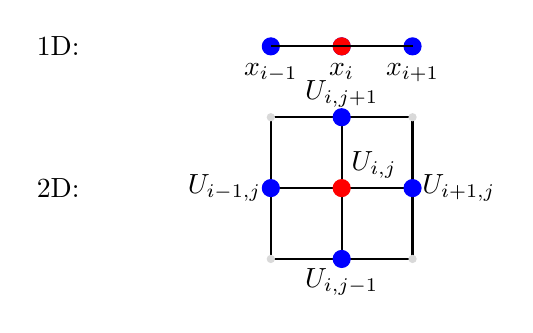
\begin{tikzpicture}[scale=0.9]
                  % 1D stencil
                  \node at (-3,1) {1D:};
                  \foreach \x in {0,1,2}
                  \filldraw[blue] (\x,1) circle (0.12);
                  \filldraw[red] (1,1) circle (0.12);

                  \draw[thick] (0,1) -- (2,1);
                  \node[below] at (0,0.9) {$x_{i-1}$};
                  \node[below] at (1,0.9) {$x_i$};
                  \node[below] at (2,0.9) {$x_{i+1}$};

                  % 2D stencil
                  \node at (-3,-1) {2D:};
                  \draw[thick,step=1] (0,-2) grid (2,0);

                  \foreach \x in {0,1,2}
                  \foreach \y in {-2,-1,0}
                  \filldraw[gray!30] (\x,\y) circle (0.05);

                  \filldraw[blue] (0,-1) circle (0.12);
                  \filldraw[blue] (2,-1) circle (0.12);
                  \filldraw[blue] (1,0) circle (0.12);
                  \filldraw[blue] (1,-2) circle (0.12);
                  \filldraw[red] (1,-1) circle (0.12);

                  \node[left] at (0,-1) {$U_{i-1,j}$};
                  \node[right] at (2,-1) {$U_{i+1,j}$};
                  \node[above] at (1,0) {$U_{i,j+1}$};
                  \node[below] at (1,-2) {$U_{i,j-1}$};
                  \node[above right] at (1,-1) {$U_{i,j}$};
              \end{tikzpicture}
              \caption{Illustration of the five-point stencil in 1D (top) and 2D (bottom). The red node is the point where the Laplacian is approximated, and blue nodes are its neighbors contributing to the finite difference formula. In 1D, a three-point stencil (red with two blue neighbors) gives the second derivative; in 2D, the four neighbors form the five-point Laplacian stencil. These central-difference formulas are accurate to $O(h^2)$ and lead to linear equations relating each interior point's value to its adjacent values.}
          \end{figure}

    \item \textbf{Formulate Interior Equations:} For each interior grid point $1\le i\le N-1$, $1\le j\le P-1$, write
          $$
              - \frac{U_{i+1,j}+U_{i-1,j}+U_{i,j+1}+U_{i,j-1}-4U_{i,j}}{h^2} = f(x_i,y_j).
          $$
          simplify to $-U_{i-1,j} - U_{i+1,j} - U_{i,j-1} - U_{i,j+1} + 4U_{i,j} = h^2 f(x_i,y_j)$.
          This yields a linear system $A\mathbf{U}=\mathbf{F}$ where $A$ is a large sparse matrix (with a typical 5-point pattern structure). You are not expected to invert $A$ by hand on an exam, but you should be able to set up the equations or write the matrix in block form. (For instance, $A$ often appears as a Kronecker sum of 1D Laplace matrices.)
    \item \textbf{Apply Boundary Conditions:}
          \begin{itemize}
              \item Dirichlet: For any boundary grid point, set $U$ to the given boundary value. These values are then treated as known in neighboring interior equations. Effectively, for each interior equation adjacent to a boundary, move the term involving the boundary neighbor to the RHS. Example: if the domain is $0\le i\le N$, $0\le j\le P$ and the top boundary ($j=P$) has Dirichlet values $U_{i,P}=g_i$, then the equation at $(i,P-1)$ includes a term $U_{i,P}$ which should be replaced by $g_i$ and brought to RHS.
              \item Neumann: For a Neumann boundary (say the top edge has $\partial u/\partial y = 0$ or some flux), use a one-sided difference normal to the boundary. For a horizontal boundary, $\partial u/\partial y \approx (U_{i,P} - U_{i,P-1})/\Delta y$ (backward difference if pointing inward) and set that equal to the specified value. Using a zero-flux example: $\frac{U_{i,P} - U_{i,P-1}}{h} = 0$ implies $U_{i,P} = U_{i,P-1}$. In practice, this allows you to eliminate the ghost node by copying the interior value: the unknown just outside the domain equals the last interior value.
              \item Mixed boundaries: Treat each side of the domain according to its type (Dirichlet or Neumann as above). If a corner has two Neumann sides, you might need a combination (but often one can handle corners by applying one boundary after the other, or a second-order accurate diagonal ghost formula if needed — usually not required unless high accuracy at corners matters).
          \end{itemize}
    \item \textbf{Solve or Outline Solution:} In an exam setting, you might not solve the full 2D system by hand (unless $N,P$ are very small). Instead, outline an approach: e.g. use iterative methods (Gauss--Seidel or Successive Over-Relaxation) to relax the interior points until convergence, or mention that the matrix $A$ can be solved by splitting it into smaller 1D problems if using separation (Fourier methods) or by employing software for large linear systems. Key is to demonstrate you know the linear system structure and properties (symmetric positive-definite for Poisson’s equation with Dirichlet BCs, so solvable and well-conditioned as $h\to0$).
    \item \textbf{Check Consistency \& Error:} The local truncation error of the 5-point Laplacian is $O(h^2)$ if $u$ is smooth, so the scheme is consistent. For convergence, typically one can argue by the Lax--Richtmyer Equivalence Theorem (here essentially showing $A$ is non-singular and stable under refinement, and truncation $\to0$ implies $|U - u| \to 0$).
          Another approach is the Discrete Maximum Principle (DMP): for Laplace’s equation ($f=0$), if $U$ violates the maximum principle then it indicates error. One can prove that the discrete solution’s maximum lies on the boundary (similar to continuous case), ensuring stability. Moreover, one can derive max-norm error bounds: for example, using the DMP and a barrier function, one can show $|e|\infty \le C h^2 |u^{(4)}|\infty$ for Poisson (meaning second-order convergence in infinity norm). Such proofs often involve comparing the discrete operator $L_h U$ applied to the error with the continuous operator on $u$, and using the invertibility of $L_h$ (via Green’s function or energy methods) to bound the error by the truncation error.
\end{enumerate}

\paragraph{Common Mistakes (2D Stationary):}
\begin{itemize}
    \item \textbf{Incorrect Stencil Application:} Writing the Laplacian difference incorrectly (e.g. missing a factor or using 4 instead of $-4$) is a common error. Always double-check the 5-point formula sign and coefficients. A quick check: for Laplace’s equation ($f=0$), the formula $U_{i+1,j}+U_{i-1,j}+U_{i,j+1}+U_{i,j-1}-4U_{i,j}=0$ means the center value is the average of its four neighbors\cite{leifh}. If your equation can’t be rearranged to $U_{i,j} = \frac{1}{4}(U_{i+1,j}+U_{i-1,j}+U_{i,j+1}+U_{i,j-1})$, it’s likely wrong.
    \item \textbf{Boundary Misapplication:} In 2D it’s easy to mix up boundary indexing. Clearly identify which grid indices lie on each boundary and apply the correct boundary formula. A mistake would be using a Neumann formula on a side that is actually Dirichlet or using the wrong neighbor for a derivative. Sketching the grid and marking boundary conditions helps avoid this.
    \item \textbf{Corner Conditions:} Corners with mixed BCs can be tricky. A common oversight is double-counting or ignoring a corner condition. If one side is Dirichlet and adjacent side Neumann, the corner node has its value from Dirichlet (that takes precedence), and the Neumann condition applies along the edge away from the corner. Don’t introduce a ghost at a Dirichlet corner -- the Dirichlet value is already known.
    \item \textbf{Large Linear System Handling:} Some students try to invert the full matrix explicitly, which is impractical. Instead, focus on describing the matrix or solution method. Not articulating how you’d solve/iterate can cost points; mention known methods (Jacobi, Gauss--Seidel, etc.) and their typical convergence for Poisson problems.
\end{itemize}

\subsection{Time-Dependent Problems: Heat/Diffusion Equation (Parabolic PDE)}
The heat equation represents diffusion processes and is first-order in time and second-order in space. We consider 1D and 2D cases. Finite difference schemes involve time-stepping. Key considerations are time step size (stability) and the method (explicit vs implicit).
\paragraph{General Heat Equation form:}
$u_t = \alpha, \Delta u + s(x,t)$ (with $\alpha>0$ the diffusion coefficient, and possibly source term $s$). Commonly, $s=0$ for pure diffusion. Initial condition $u(x,0)=f(x)$ is given, along with BCs (Dirichlet: fixed temperature, or Neumann: insulated, etc.).
\subsubsection{1D Heat Equation (Explicit and Implicit Schemes)}
\paragraph{Problem Setup:}
$u_t = \alpha, u_{xx}$ for $x\in[a,b]$, $t>0$, with initial profile $u(x,0)=f(x)$. Boundary conditions can be Dirichlet (e.g. $u(a,t)=A(t)$, $u(b,t)=B(t)$ fixed in time) or Neumann ($u_x(a,t)=0$ insulated end, etc.). We seek $U_j^n \approx u(x_j, t^n)$ on a space grid $x_j = a + j\Delta x$ ($j=0,\dots,N$) and time levels $t^n = n\Delta t$.
\paragraph{Solution Recipe (Step-by-Step):}
\begin{enumerate}
    \item \textbf{Choose a Time-Stepping Scheme:} Decide between an explicit method (easy but conditionally stable) or an implicit method (unconditionally stable but requires solving linear systems each step). Two common schemes:
          \begin{itemize}
              \item Forward Time, Centered Space (FTCS) -- explicit Euler in time, central difference in space.
              \item Backward Time, Centered Space (BTCS) -- implicit Euler in time, central in space.
              \item Crank--Nicolson (CN) -- trapezoidal rule (average of explicit/implicit), which is unconditionally stable and second-order accurate in time.
          \end{itemize}
    \item \textbf{Set Up the Grid:} Let $\Delta x = (b-a)/N$ and $\Delta t$ be chosen (possibly from a stability criterion). Define grid values $U_j^n \approx u(x_j, t^n)$. Incorporate initial condition: set $U_j^0 = f(x_j)$ for all $j$.
    \item \textbf{Write the Finite Difference Update:} For FTCS (explicit), use forward difference in time and central in space:
          $$\frac{U_j^{n+1}-U_j^n}{\Delta t} = \alpha\frac{U_{j+1}^n - 2U_j^n + U_{j-1}^n}{\Delta x^2},$$ which rearranges to the explicit update formula:
          $$U_j^{n+1} = U_j^n + \underbrace{\frac{\alpha\Delta t}{\Delta x^2}}_{=:r}\left(U_{j+1}^n - 2U_j^n + U_{j-1}^n\right).$$
          Here $r = \frac{\alpha\Delta t}{\Delta x^2}$ is the \textbf{diffusion Courant number} (ratio controlling stability)\cite{ddcampayo}.
          This scheme is first-order accurate in time, second-order in space.
          \medskip
          For BTCS (implicit), use backward time and central space:
          $$\frac{U_j^{n+1}-U_j^n}{\Delta t} = \alpha\frac{U_{j+1}^{n+1} - 2U_j^{n+1} + U_{j-1}^{n+1}}{\Delta x^2},$$
          leading to a linear system at each time step:

          $$-rU_{j-1}^{n+1} + (1+2r) U_j^{n+1} - rU_{j+1}^{n+1} = U_j^n$$

          for all interior $j$.
          This is unconditionally stable and first-order in time.

          \medskip

          For Crank--Nicolson, average the RHS of explicit and implicit (or equivalently trapezoidal rule in time):

          \[
              \frac{U_j^{n+1}-U_j^n}{\Delta t} = \frac{\alpha}{2}\left(\frac{U_{j+1}^{n+1} - 2U_j^{n+1} + U_{j-1}^{n+1}}{\Delta x^2} + \frac{U_{j+1}^n - 2U_j^n + U_{j-1}^n}{\Delta x^2}\right),
          \]
          This yields a linear system (like implicit) but with improved second-order time accuracy:
    \item \textbf{Apply Boundary Conditions Each Step:}
          \begin{itemize}
              \item Dirichlet BC: Simply enforce $U_0^n = A(t^n)$ and $U_N^n = B(t^n)$ at each time step $n$. In the explicit formula, you’ll need $j-1$ or $j+1$ that might be a boundary -- use the known value. In implicit systems, the known boundary values move to the RHS of the linear system.
              \item Neumann BC: Use ghost points or one-sided differences at the boundaries for spatial derivatives. For example, if $u_x(a,t)=0$, approximate $\frac{U_1^n - U_{-1}^n}{2\Delta x}=0$ implying $U_{-1}^n = U_1^n$. In an explicit update for $j=0$, you would use $U_{-1}^n = U_1^n$ when computing $U_0^{n+1}$. For implicit, the boundary equation can be formulated using the one-sided second derivative: e.g. $\frac{U_2^{n+1}-2U_1^{n+1}+U_0^{n+1}}{\Delta x^2}$ with $U_0$ and ghost relation $U_0^{n+1}=U_2^{n+1}$ (since $U_0$ and $U_{-1}$ symmetric about boundary) for a zero-flux left boundary. This effectively modifies the first row of the linear system.
              \item Periodic BC: (If applicable) equate $U_0^n = U_N^n$ and similarly $U_{-1}^n = U_{N-1}^n$ etc., whenever using neighbors across the boundary.
          \end{itemize}
    \item \textbf{March in Time:}
          \begin{itemize}
              \item For explicit schemes, iterate the update for $n=0,1,2,\dots$ until the desired final time.
              \item Stability check: ensure the time step satisfies the CFL (Courant--Friedrichs--Lewy) condition.
              \item For FTCS on the heat equation, the stability criterion is $r = \frac{\alpha \Delta t}{\Delta x^2} \le \frac{1}{2}$ (in fact, $r=1/2$ is the borderline case)\cite{ddcampayo}.
              \item This comes from von Neumann analysis requiring $|1-4r\sin^2(\frac{k\Delta x}{2})|\le 1$ for all Fourier modes, whose worst-case ($\sin^2=1$) gives $|1-2r|\le 1$, i.e. $r\le 1/2$.

              \item Always check this before trusting an explicit simulation -- too large a $\Delta t$ will cause the solution to blow up (unbounded oscillatory growth of errors).

              \item If the criterion is violated, choose a smaller $\Delta t$ or switch to an implicit method.
                    \medskip
              \item For implicit schemes (BTCS, CN), no such strict constraint exists; they are unconditionally stable, so you can take larger time steps (limited only by accuracy considerations, not stability).
          \end{itemize}
    \item \textbf{Solve Linear Systems if Needed:} For BTCS or Crank--Nicolson, at each step solve the tri-diagonal linear system for $U^{n+1}$. On an exam, you might be asked to set up this system or possibly perform one step of solving it (e.g. via Gaussian elimination or the Thomas algorithm for a small $N$). You should also note the matrix structure (e.g. $(1+2r)$ on diagonal and $-r$ on off-diagonals for BTCS).
    \item \textbf{Stability \& Convergence Analysis:}
          \begin{itemize}
              \item To \textbf{check consistency}, derive the truncation error by plugging the exact solution’s Taylor expansions: e.g. for FTCS, $U_j^{n+1}-U_j^n = \Delta t, u_t + \frac{(\Delta t)^2}{2}u_{tt} + ...$, and $U_{j+1}^n - 2U_j^n + U_{j-1}^n = \Delta x^2 u_{xx} + \frac{(\Delta x)^4}{12}u_{xxxx}+...$. You’ll find the local truncation error is $O((\Delta t) + (\Delta x)^2)$, so the scheme is first-order in time, second in space. CN would yield $O((\Delta t)^2 + (\Delta x)^2)$.
              \item For \textbf{stability}, use \textbf{von Neumann analysis}: assume a mode $U_j^n = G^n e^{i k x_j}$, substitute in the scheme to find the amplification factor $G$ as a function of $k\Delta x$ and $r$. Require $|G|\le 1$ for all $k$. We did this above for FTCS, getting $|G| = |1 - 4r\sin^2(\frac{k\Delta x}{2})|$ and demanding it $\le 1$ which gave $r\le 1/2$. For BTCS, you’d get an amplification factor $G = \frac{1}{1+4r\sin^2(\frac{k\Delta x}{2})}$, whose magnitude is always $<1$ for any $r>0$ (hence unconditionally stable). Knowing how to set up this analysis is useful if asked.
              \item \textbf{Convergence}: If a scheme is consistent and stable, it will converge (Lax equivalence theorem). To be thorough without invoking Lax, one can sometimes do an energy norm analysis: e.g. multiply the error evolution equation by the error and integrate (discrete analog of an $L^2$ energy) to show error decays or stays bounded by the initial error plus truncation terms. On an exam, a common task is to show something like $\max_{m\le M, n\le N} |e_j^n| \le C(\Delta t^p + \Delta x^q)$ given a truncation error bound $|\tau_j^n| \le C'((\Delta t)^p + (\Delta x)^q)$
              \item Hints: use induction in time steps and the fact that stability gives a bound on error growth. For implicit methods, often you can show the matrix is diagonally dominant or use the matrix norm to bound the amplification per step by 1, then sum up the truncation contributions.
          \end{itemize}
\end{enumerate}

\paragraph{Common Mistakes (Heat Equation):}
\begin{itemize}
    \item \textbf{Violating Stability (Explicit):} The most frequent pitfall is using an unstable time step. Remember $r \le 1/2$ (for 1D) is essential. If you see weird oscillations or increasing error in a test computation, likely $\Delta t$ is too large. Always mention the CFL condition when discussing explicit schemes.

    \item \textbf{Boundary Condition Implementation:} In updating the first and last grid point, ensure you properly use BCs. E.g., a student might mistakenly update $U_0^{n+1}$ using the interior formula, not realizing $U_{-1}$ is outside domain -- you must use the boundary condition at $j=0$. For Dirichlet, it means $U_0^{n+1}$ is fixed (no update needed, just assign the BC value); for Neumann, use the ghost node elimination as described.

    \item \textbf{Indexing in Time:} Mixing up $U_j^{n}$ and $U_j^{n+1}$ on the RHS is another error. Write down clearly whether you're using values from the old time level or new. For implicit schemes, don't use $U^n$ on the RHS of spatial second derivative for BTCS (that would make it explicit!). In BTCS, all spatial terms should be at $n+1$.

    \item \textbf{Solving Implicit Systems:} If deriving Crank--Nicolson, students sometimes end up with an incorrect time-centering. Double-check the algebra: CN should produce terms like $U^n$ and $U^{n+1}$ averaged. A mistake here can lead to a scheme that's not actually second-order. Also, when solving the linear system, ensure you include the RHS contributions from $U^n$ properly.

    \item \textbf{Not Updating the Entire Domain:} It's easy to forget to update the interior only and handle boundaries separately. Make sure you clarify that for each time step: you update all interior $j=1,\ldots,N-1$ via the scheme, and then immediately impose boundary values for $U_0^{n+1},U_N^{n+1}$ (either copying Dirichlet values or applying Neumann formula). This two-step (interior update + BC application) ensures the boundary at the new time is correct.
\end{itemize}

\subsubsection{2D Heat Equation}
The extension to two spatial dimensions follows similarly, but there are a few added concerns with stability and complexity:
\paragraph{Key Differences from 1D:}
\begin{itemize}
    \item The Laplacian now has second differences in both $x$ and $y$. For example, an explicit scheme on a uniform square grid ($h = \Delta x = \Delta y$) looks like:
          $$U_{i,j}^{n+1} = U_{i,j}^n + r \Big(U_{i+1,j}^n + U_{i-1,j}^n + U_{i,j+1}^n + U_{i,j-1}^n - 4U_{i,j}^n\Big),$$
          with $r = \alpha\Delta t/h^2$.
    \item The stability condition for 2D FTCS is more severe: the criterion becomes $r \le 1/4$ (since the highest-frequency error mode can grow faster in two dimensions). In general, for an explicit diffusion in $d$ dimensions, $r \le 1/(2d)$ is required.
    \item Implicit methods (like BTCS or CN) in 2D lead to larger linear systems (with a 5-point stencil coupling). These can be solved by iterative solvers or matrix factorizations (though direct solve is $O(N^3)$ which is expensive; in practice one might use techniques like ADI -- Alternating Direction Implicit -- splitting the 2D solve into two 1D solves per step, but that’s beyond exam scope unless taught).
\end{itemize}

\paragraph{Steps (briefly):}
\begin{itemize}
    \item Set up a grid $(i,j)$ for $i=0...N$, $j=0...P$. Impose initial condition $U_{i,j}^0 = f(x_i,y_j)$.
    \item Choose scheme: explicit FTCS as above, or implicit where each time step requires solving a 2D Poisson-type equation $(I + rL_h)U^{n+1} = U^n$ (for BTCS).
    \item Apply boundary conditions similarly: for each side (Dirichlet: set edges directly; Neumann: use ghost layer and one-sided differences for normal derivative).
    \item Check stability: For explicit, ensure $r \le 1/4$ (if $\Delta x = \Delta y$) -- in general the formula is $r \le \frac{1}{2}\frac{1}{1 + (\Delta x/\Delta y)^2}$ for a rectangle (worst-case error mode is a checkerboard alternating in both $x$ and $y$ directions). If using equal spacings, this simplifies to $r\le 1/4$. Implicit schemes are unconditionally stable in 2D as well.
    \item March in time or solve implicit steps as needed. If using CN in 2D, one strategy is to use an ADI method to split the 2D system into two 1D systems per half-step (this avoids solving a full NxN linear system directly). If the exam covers ADI, outline its steps; otherwise, a generic mention of solving via iterative methods (Gauss--Seidel, multigrid, etc.) is fine.
\end{itemize}

\paragraph{Common Mistakes (2D Heat):}
\begin{itemize}
    \item Using 1D Stability Limit: Don’t forget that 2D explicit diffusion has a stricter condition. Students sometimes use $\Delta t = \frac{\Delta x^2}{2\alpha}$ (1D limit) in a 2D problem, which is too large by roughly a factor of 2. Always adjust for number of spatial dimensions: for 2D, $\alpha\Delta t(\frac{1}{\Delta x^2}+\frac{1}{\Delta y^2}) \le 1/2$ is the general stability requirement (for equal spacing, that gives $\alpha \Delta t/h^2 \le 1/4$).
    \item Iterative Solve Missteps: If asked how to solve the implicit 2D system, avoid hand-waving “just invert the matrix” -- mention a plausible method. A mistake is to treat the 2D matrix as tridiagonal (it’s block tridiagonal); one can say “use Gauss--Seidel sweeps over the grid until convergence” -- that is a legitimate approach for the heat equation steady state or backward Euler step.
    \item Boundary Condition Handling: In updating a corner explicitly, make sure you account for both directions. E.g. at $(i=1,j=1)$ near a corner with Neumann on left and bottom, the explicit update uses $U_{0,1}, U_{1,0}$ which are ghosts determined by Neumann conditions in $x$ and $y$ respectively. Don’t mix up which ghost corresponds to which derivative.
    \item Exceeding Stability in Source Terms: If a source term $s(x,t)$ is present, stability analysis changes slightly (source doesn’t affect homogeneous stability, but large source can cause fast growth of true solution). Ensure your time step also resolves source dynamics (you might need smaller $\Delta t$ to accurately capture a fast source even if mathematically stable).
\end{itemize}
\subsection{Time-Dependent Problems: Wave Equation (Hyperbolic PDE)}
The wave equation
$$
    u_{tt} = c^2 \Delta u, \text{ with } c \text{ the wave speed}
$$
is second-order in time. Unlike diffusion, it propagates waves without damping (in the ideal case).
This requires careful handling: FDM schemes often use a “leapfrog” style two-step update.

Stability is governed by the \textbf{Courant number}
$$C = c\Delta t/\Delta x.$$

We cover the standard explicit central difference scheme for wave propagation in 1D and 2D.

\subsubsection{1D Wave Equation}
\paragraph{Problem Setup:}
$u_{tt} = c^2 u_{xx}$ for $x\in[a,b]$, with initial displacement $u(x,0)=g(x)$ and initial velocity $u_t(x,0)=h(x)$. Boundary conditions might be fixed ends (Dirichlet: e.g. $u(a,t)=0, u(b,t)=0$ for a vibrating string with fixed ends) or free ends (Neumann: $u_x=0$ at boundaries, implying no spatial slope at the end, like a rod with frictionless ends).

\paragraph{Solution Recipe:}
\begin{enumerate}
    \item \textbf{Discretize Space and Time:} Use spacing $\Delta x$ and time step $\Delta t$. For convenience, denote $r = \frac{c\Delta t}{\Delta x}$ (Courant number for the wave equation). Let $U_j^n \approx u(x_j, t^n)$ with $j=0...N$ and $n=0,1,2,...$.
    \item \textbf{Finite Difference Scheme (Leapfrog):} A widely used scheme is the second-order central difference in time and space:
          $$\frac{U_j^{n+1} - 2U_j^n + U_j^{n-1}}{(\Delta t)^2} = c^2 \frac{U_{j+1}^n - 2U_j^n + U_{j-1}^n}{(\Delta x)^2}.$$
          This yields an explicit update formula solving for $U_j^{n+1}$:
          $$U_j^{n+1} = 2U_j^n - U_j^{n-1} + \lambda^2\big(U_{j+1}^n - 2U_j^n + U_{j-1}^n\big),$$
          where $\lambda = c\frac{\Delta t}{\Delta x} = r$ in 1D. This scheme is second-order accurate in both time and space. It’s essentially the discrete d’Alembert formula and is equivalent to two coupled first-order updates (for $u_t$ and $u$) in leapfrog fashion.
    \item \textbf{Initial Conditions Implementation:} Here we have two initial conditions (at $t=0$ for $u$ and $u_t$). The scheme needs $U_j^0$ and $U_j^1$ to start.
          \begin{itemize}
              \item Use the given initial displacement: set $U_j^0 = g(x_j)$.
              \item To obtain $U_j^1$ (the solution at one time-step later), use the initial velocity $h(x) = u_t(x,0)$.
                    One method is to use a \textbf{forward difference in time} for the first step: $u_t(x,0) \approx \frac{U_j^1 - U_j^0}{\Delta t}$.
                    Rearranged, $U_j^1 = U_j^0 + \Delta th(x_j) + \frac{(\Delta t)^2}{2}c^2u_{xx}(x_j, 0)$ if we want second-order accuracy. If $u_{xx}(x,0)$ is not readily known, an approximation can be made using the spatial second difference of $g(x)$: $u_{xx}(x_j,0) \approx \frac{g(x_{j+1}) - 2g(x_j) + g(x_{j-1})}{(\Delta x)^2}$.
                    Thus a practical formula is:
                    $$U_j^1 = U_j^0 + \Delta th(x_j) + \frac{1}{2}\lambda^2 \big(U_{j+1}^0 - 2U_j^0 + U_{j-1}^0\big).$$
                    This “half-step” initialization ensures $U^1$ is second-order accurate. (If initial velocity is zero, this simplifies to $U_j^1 = U_j^0 + \frac{1}{2}\lambda^2(...)$ which is basically a small adjustment from the curvature of $g$.)
          \end{itemize}
    \item \textbf{Boundary Conditions:}
          \begin{itemize}
              \item Dirichlet (fixed ends): Enforce $U_0^n = A(t^n)$ and $U_N^n = B(t^n)$ for all $n$. Often $A$ and $B$ are zero (homogeneous Dirichlet for ends fixed at zero displacement). The update formula for $j=1$ or $j=N-1$ uses $U_0$ or $U_N$ which are known, so include those as known terms. If both ends are fixed zero, note that physically the scheme will preserve certain symmetries.
              \item Neumann (free ends): Typically $u_x(a,t)=0$ translates to $\frac{U_1^n - U_{-1}^n}{2\Delta x}=0$ so $U_{-1}^n = U_1^n$. In the update formula for the end $j=0$, you’d substitute $U_{-1}^n = U_1^n$, yielding $U_0^{n+1} = 2U_0^n - U_0^{n-1} + \lambda^2 (U_1^n - 2U_0^n + U_{-1}^n)$ = $2U_0^n - U_0^{n-1} + \lambda^2 (U_1^n - 2U_0^n + U_1^n)$ = $2U_0^n - U_0^{n-1} + 2\lambda^2 (U_1^n - U_0^n)$. This effectively is a one-sided second derivative formula consistent with Neumann. Perform similar at $j=N$ using $U_{N+1}^n = U_{N-1}^n$ for zero flux.
              \item Mixed: If one end is fixed and the other free, handle each accordingly.
          \end{itemize}
    \item \textbf{Time Marching and Stability:} Use the leapfrog update for $n=1$ to $N_t-1$ to advance in time. The critical stability condition for this explicit wave scheme is
          $$\lambda = \frac{c\Delta t}{\Delta x} \;\le\; 1,$$
          i.e. $\Delta t \le \Delta x/c$. This is the CFL condition for 1D wave equations . If $\lambda>1$, the scheme becomes unstable (Fourier modes grow or decay unboundedly instead of oscillating). At $\lambda=1$, the scheme is neutrally stable (zero numerical damping, errors neither grow nor decay for ideal case). Usually one chooses a slightly smaller $\lambda$ (e.g. 0.95) to be safe. Von Neumann analysis shows the amplification factor $G = 1 - \lambda^2(1-\cos(k\Delta x))$ for this scheme leads to $|G| \le 1$ iff $\lambda \le 1$. Always check that your chosen $\Delta t$ satisfies this before computing.
    \item \textbf{Energy and Convergence:} The wave equation has a conserved energy $E = \int (\frac{1}{2}u_t^2 + \frac{c^2}{2}u_x^2)dx$. The numerical scheme similarly conserves a discrete energy when $\lambda=1$ (and slightly decays it if $\lambda<1$ due to numerical dispersion). To demonstrate convergence, one can show consistency (truncation error $O((\Delta t)^2 + (\Delta x)^2)$) and stability (CFL condition). Lax’s theorem then gives convergence. For a more direct argument, one can utilize the discrete energy method: assume a discrete solution and error, derive an equation for error energy growth. If $\lambda\le1$, show that the energy (and thus error) cannot grow in time, implying stability and convergence order matching the truncation error order.
\end{enumerate}
\paragraph{Common Mistakes (1D Wave):}
\begin{itemize}
    \item \textbf{Forgetting Second Initial Condition:} A common oversight is to start the scheme with only $U^0$ and use the update formula, which requires $U^{-1}$ (previous time step). Always compute $U^1$ using the initial velocity info. If you neglect to properly initialize $U^1$, the scheme effectively becomes first-order or can even start with incorrect oscillations. Use the formula provided to include $h(x)$.
    \item \textbf{Stability Neglect:} It’s easy to assume any small $\Delta t$ is fine. But “small” is relative; if $\Delta t$ doesn’t satisfy $c\Delta t < \Delta x$, the solution will blow up. For example, if you halve $\Delta x$ but keep $\Delta t$ same, the scheme may become unstable. Always adjust $\Delta t$ with grid refinement to keep $\lambda$ in range.
    \item \textbf{Boundary Reflections and Implementation:} When using Neumann BC, a mistake is to treat the ghost as equal to the interior point (which is correct for zero flux) but then also apply a Dirichlet update — double-dipping. Use either the ghost point method in the stencil or derive a special formula for boundary update; don’t impose conflicting conditions. If boundaries are time-dependent (e.g. oscillating end), make sure to insert those values at each time step directly rather than computing them via the interior formula.
    \item \textbf{Index Mist in Update:} The wave update couples $n+1$ with $n-1$. Some students incorrectly write it as $U_j^{n+1} = U_j^{n-1} + ...$ (dropping the $2U_j^n$ term). Remember the correct form has both the previous time step and the current one: it’s effectively $U^{n+1} - 2U^n + U^{n-1} = \lambda^2(...)$. Write it out carefully and, if unsure, derive it by applying the second-time finite difference approximation to $u_{tt}=c^2u_{xx}$.
    \item \textbf{Interpretation of $\lambda=1$ Case:} If $\lambda$ is exactly 1, the scheme is neutrally stable — errors neither grow nor dissipate (in theory). In practice, floating-point rounding can then accumulate. It’s safer to run with $\lambda$ slightly below 1. On an exam, if asked for the “stability limit”, give $\lambda \le 1$, but if asked for strict stability vs neutral, you might say $\lambda<1$ for strict stability and $\lambda=1$ is the borderline case.
\end{itemize}



\subsubsection{2D Wave Equation}
For a domain in 2D, e.g. $u_{tt} = c^2(u_{xx}+u_{yy})$, the finite difference is analogous but each point's update involves its four nearest neighbors in space:
$$\frac{U_{i,j}^{n+1} - 2U_{i,j}^n + U_{i,j}^{n-1}}{(\Delta t)^2} = c^2 \Big(\frac{U_{i+1,j}^n - 2U_{i,j}^n + U_{i-1,j}^n}{\Delta x^2} + \frac{U_{i,j+1}^n - 2U_{i,j}^n + U_{i,j-1}^n}{\Delta y^2}\Big).$$

If using equal spacing $h = \Delta x = \Delta y$, this simplifies to:
$$U_{i,j}^{n+1} = 2U_{i,j}^n - U_{i,j}^{n-1} + \lambda^2 \Big(U_{i+1,j}^n + U_{i-1,j}^n + U_{i,j+1}^n + U_{i,j-1}^n - 4U_{i,j}^n\Big),$$
with $\lambda = c\Delta t/h$. Initial conditions $U_{i,j}^0 = g(x_i,y_j)$ and $U_{i,j}^1$ computed similarly using $h(x,y)$ (initial velocity field) and second spatial derivatives. Boundary conditions (Dirichlet or Neumann) are applied on all edges of the 2D grid (and ghost layers for Neumann as in the heat eq 2D case).

\paragraph{Stability in 2D:} The condition is stricter: the CFL condition becomes
$$\lambda \le \frac{1}{\sqrt{2}}$$
for equal grid spacing. In general, for a grid spacing $(\Delta x,\Delta y)$, stability requires $c^2\Delta t^2\Big(\frac{1}{\Delta x^2}+\frac{1}{\Delta y^2}\Big) \le 1$. Intuitively, the shortest wavelength mode in 2D can oscillate in both $x$ and $y$ directions simultaneously, so the time step must be small enough to handle variation in both directions. For example, if $\Delta x = \Delta y$, this condition reduces to $c\Delta t/h \le 1/\sqrt{2} \approx 0.707$. If one spacing is finer than the other, the stricter requirement comes from that (the formula above covers it).

\paragraph{Other aspects:} Solving 2D wave equations usually means updating a big grid every time step -- which is feasible explicitly. If the exam problem is theoretical, stick to writing the scheme and stating the stability condition. If it's practical (simulate something), mention how you'd enforce boundary conditions each step (similar to 1D, applied along each edge).

\paragraph{Common Mistakes (2D Wave):}
\begin{itemize}
    \item \textbf{Using 1D CFL in 2D:} As with heat, using $\lambda \le 1$ in multi-D wave is dangerous. Always include the $\frac{1}{\sqrt{2}}$ factor for 2D (or $\frac{1}{\sqrt{3}}$ for 3D, in general $\lambda \le 1/\sqrt{\text{spatial dims}}$ for the standard 3-point/time, 5-point/space scheme).

    \item \textbf{Corner Handling:} If you have Neumann edges, the corner of a 2D domain requires consistency in both directions. Some might attempt to use a diagonal ghost which gets complicated. A simpler approach: apply the horizontal Neumann for the corner in the horizontal neighbor, and vertical for the vertical neighbor -- effectively the corner value gets updated using the interior formula plus ghost substitutions from both sides. If unsure, you can also treat the corner as having a Neumann condition in both directions (meaning reflect across both axes: $U_{-1,-1} = U_{1,1}$ for a corner with Neumann on left and bottom, etc.). However, typically exam problems avoid double-Neumann corners or accept a physically reasonable handling.

    \item \textbf{Polar or Irregular Domains:} Sometimes wave equations might be in a circular membrane etc. If not specifically asked, do not venture into non-Cartesian grids -- stick to the given domain. If asked, you might need to transform or use approximations (but that's advanced).

    \item \textbf{Memory of Past Step:} Because the wave scheme uses $n-1$, one must store two past time slices. A trivial mistake is to always update from the same array, inadvertently using $U^{n}$ and $U^{n-1}$ that were overwritten. In practice, use two arrays (or three rotating) for $U^{n+1},U^n,U^{n-1}$. When writing pseudo-code or explaining, be clear on how $U^{n-1}$ is retained.

    \item \textbf{Over-damped Behavior:} If someone mistakenly adds a term like $U_j^{n-1}$ with a plus sign (instead of minus) or uses an incorrect coefficient, the scheme could become overly diffusive or unstable. Double-check the derived scheme by testing simple cases: e.g., constant solution $u=\text{const}$ should remain constant ($U_j^{n+1}=U_j^n$); one spatial oscillation ($(-1)^j$ pattern) should produce the appropriate oscillation in time given the CFL chosen.
\end{itemize}

\subsection{Analysis and Verification Tasks}

\subsubsection{Truncation Error \& Consistency}

\paragraph{Truncation Error:}
To derive the local truncation error $\tau$, assume the solution $u(x,t)$ is sufficiently smooth. Write out the Taylor series for terms in your scheme. For example, in 1D, for a point $x_j$:
$$u(x_{j+1}, t) = u + h u_x + \frac{h^2}{2}u_{xx} + \frac{h^3}{6}u_{xxx} + \frac{h^4}{24} u_{xxxx} + \ldots$$
Similarly $u(x_{j-1},t)$ expands with $-h$.

Use these to replace $U_{j+1}^n, U_{j-1}^n$ by $u$ plus derivatives, and likewise for time expansions (e.g. $u(t+\Delta t) = u + \Delta tu_t + \frac{\Delta t^2}{2}u_{tt} + \ldots$).

Plug the exact $u$ expansions into the difference scheme formula and cancel out terms that correspond to the PDE $u_{t}, u_{xx}$ etc. Whatever remains (typically the first neglected term) is $\tau$.

For instance, for the heat FTCS scheme, after substituting expansions you might get $\tau \sim \frac{\Delta t}{2}u_{tt}(x_j,t^n) - \frac{\Delta x^2}{12}u_{xxxx}(x_j,t^n) + \ldots$. Using the PDE $u_{tt} = \alpha u_{xx}$ to eliminate $u_{tt}$, you'd find $\tau = O(\Delta t) + O(\Delta x^2)$. State the leading term and order.

\paragraph{Consistency:} If the truncation error $\tau \to 0$ as $\Delta t, \Delta x \to 0$, the scheme is consistent with the PDE. Simply put, make sure your finite difference equation formally approaches the PDE for small step sizes. (All schemes we discussed are consistent of at least first order.)

\subsubsection{Stability (von Neumann analysis)}
\paragraph{Procedure:}
\begin{enumerate}
    \item Assume linear PDE and linear scheme (no nonlinear terms for von Neumann).

    \item Take an ansatz $U_{j}^n = \zeta^n e^{i k x_j}$ (Fourier mode with wavenumber $k$).

    \item Substitute into the finite difference update equation.

    \item The spatial difference operators acting on $e^{i k x_j}$ will yield factors like $e^{i k x_{j+1}} = e^{i k h}e^{i k x_j}$, etc.

    \item Factor out $e^{i k x_j}$ and cancel it.

    \item Solve the resulting equation for $\zeta$, the amplification factor per time step:
          $$\mathcal{Q}(\zeta, e^{ik h}) = 0,$$
          where $\mathcal{Q}$ is a polynomial. (Note: it may be a quadratic for schemes like wave eq).
\end{enumerate}

\begin{example}{Von Neumann for FTCS heat equation:}
    For the heat FTCS, one gets $\zeta = 1 + \alpha \Delta t \frac{e^{i k h} - 2 + e^{-i k h}}{\Delta x^2} = 1 - 2r + 2r\cos(kh)$, so $\zeta = 1 - 4r\sin^2(\frac{k h}{2})$. For stability we need $|\zeta| \le 1$ for all $k$.

    This gives the condition on $r$. If the scheme yields $|\zeta| \le 1$ only under certain step size conditions, that's the CFL condition; if it always $\le1$ (like implicit heat or conservative wave at CFL=1), then it's unconditionally stable in the linear analysis sense.

\end{example}

For multi-dimensional or multi-step schemes, you might get a condition like $|\zeta|^2 = 1 - \text{(positive expression)}$. That automatically $\le1$ if the expression is $\ge0$. This often leads to the CFL requirement. For instance, 2D wave gives $|\zeta|^2 = 1 - \lambda^2[ \sin^2(kh/2)+\sin^2(lh/2) ]$. Requiring this $\le1$ yields $\lambda^2[ \sin^2(...)+\sin^2(...) ] \le 1$ for all $k,l$, worst-case when sin terms $=1$: $\lambda^2(1+1)\le1$ i.e. $\lambda \le 1/\sqrt{2}$.

\paragraph{Boundary effects:} Note that von Neumann assumes an infinite or periodic domain (ignores boundaries). It checks internal stability. If a scheme is von Neumann stable and you apply proper boundary conditions, usually the scheme is stable in the whole domain. Only pathological boundary treatments can cause issues beyond von Neumann (like reflection amplifications, etc., which are rare in standard BCs).

\subsubsection{Convergence \& Error Bounds}

\paragraph{Convergence:}
\begin{theorem}{Lax's Equivalence}{}
    For linear initial value problems, consistency + stability = convergence.

    $$\boxed{\text{If } \tau \to 0 \text{ and } |\zeta| \le 1, \text{ then } \|U_j^n - u(x_j,t^n)\| \to 0 \text{ as } \Delta x, \Delta t \to 0.}$$
\end{theorem}
Thus, if you have shown your scheme is consistent (small truncation error) and stable (errors don't blow up), you can conclude the scheme's solution $U_j^n$ approaches the true $u(x_j,t^n)$ as $\Delta x, \Delta t \to 0$. In exam answers, after showing consistency and citing von Neumann stability, it is usually enough to state by Lax's theorem the scheme is convergent of the same order as its truncation error.

\paragraph{Order of Convergence:} Often, you might be asked to verify the order by numerical experiment or derivation. The truncation error's leading term tells you the local error per step. If it's $O(h^p) + O(\Delta t^q)$, typically the scheme is globally $O(h^p + \Delta t^q)$ (assuming stability). For example, CN scheme has local error $O((\Delta t)^3)$ and $O(h^2)$, but global error $O((\Delta t)^2 + h^2)$ (since it's second-order in time globally). Be clear on this distinction if needed: local truncation order vs global convergence order.

\paragraph{Maximum Norm Error Bounds:} For elliptic (stationary) problems, one technique is using the Discrete Maximum Principle as mentioned to bound errors. Outline: if $L_h U = f_h$ and $L u = f$ (continuous), let $e_h = U - P_h u$ (difference between numerical and interpolated exact solution). Then $L_h e_h = \tau_h$ (discretization error). Using the inverse of $L_h$ (like a Greens function argument or energy norms), one can often show $|e_h|_\infty \le C |\tau_h|_\infty$. Since $\tau_h = O(h^p)$, this gives $|e_h|_\infty = O(h^p)$. A simpler way in answers: say "Because the finite difference scheme is second-order accurate and the discrete operator is stable (e.g., satisfies a maximum principle), we have $\max|U_i - u(x_i)| \le C h^2$ for some constant $C$".

\paragraph{Energy Norms for Parabolic/Hyperbolic:} For heat/wave, sometimes you can derive an energy inequality. E.g., for heat implicit, show $(U^{n+1} - u(t^{n+1}), A (U^{n+1}-u(t^{n+1}))) \le (\text{old error term})^2 + (\text{truncation term})^2$ where $A$ is positive-definite matrix from Laplacian. Without going too deep, you can assert that such schemes are stable in $L^2$ norm, hence errors are bounded by accumulated truncation.

\paragraph{Practical error estimation:} If asked how to estimate error in a computation, a strategy is grid refinement: run the simulation with step sizes $(h, \Delta t)$ and then with $(h/2, \Delta t/2)$ and compare results -- the difference approximates the error and should scale by $\approx 2^p$ if $p$-th order (this is Richardson extrapolation idea).

\subsubsection{Common Pitfalls in Analysis}

\begin{itemize}
    \item \textbf{Mixing up Stability vs Convergence:} Don't say "scheme is stable so it's accurate" -- stability means bounded growth of errors, but you also need consistency for accuracy. Always mention both for convergence.

    \item \textbf{Incorrect Fourier Mode Ans\"atze:} Make sure to include the factor $e^{ikx_j}$ and the time growth $\zeta^n$. Some forget $\zeta^n$ and end up analyzing spatial Fourier series instead of growth. The proper substitution is $U_j^n = \hat{G}^n e^{i k j h}$ (where $\hat{G}$ is often written as $e^{\sigma \Delta t}$ or so). After canceling, you solve for $\hat{G}$.

    \item \textbf{Ignoring Nonlinear terms:} Von Neumann is for linear equations. If you have a nonlinear term (like $u u_x$ in Burgers' eq), von Neumann doesn't directly apply. You might linearize or use energy methods. On an exam, if faced with a nonlinear stability question, often the answer is "use Fourier analysis on the linear part, and note that nonlinear term doesn't produce new growth of high-frequency if treated properly" or use a modified approach (maybe not in this course).

    \item \textbf{Not answering what's asked:} If the question says "show stability without using Lax theorem," they probably expect an energy method or induction argument. Pay attention to such hints (like where they hinted at not invoking Lax). In that case, demonstrate $|U^n - u^n| \le (1+ \text{something})\cdot|U^{n-1}-u^{n-1}| + \text{const}\cdot(\text{truncation})$ and then conclude via Gronwall or induction that error stays bounded and small.
\end{itemize}

% print the bibliography biblatex
\printbibliography
\end{document}
